%%%%%%%%%%%%%%%%%%%%%%%%%%%%%%%%%%%%%%%%%%%%%%%%
%% Intro to LaTeX and Template for Homework Assignments
%% Quantitative Methods in Political Science
%% University of Mannheim
%% Fall 2017
%%%%%%%%%%%%%%%%%%%%%%%%%%%%%%%%%%%%%%%%%%%%%%%%



% This template and tutorial will help you to write up your homework. It will also help you to use Latex for other assignments than this course's homework.

%%%%%%%%%%%%%%%%%%%%%%%%%%%%%%%%%%%%%%%%%%%%%%%%
% Before we get started
%%%%%%%%%%%%%%%%%%%%%%%%%%%%%%%%%%%%%%%%%%%%%%%%

% Make an account on overleaf.com and get started. No need to install anything.

%%%%%%%%%%%%%%%%%%%%%%%%%%%%%%%%%%%%%%%%%%%%%%%%
% Or if you want it the nerdy way...
% INSTALL LATEX: Before we can get started you need to install LaTeX on your computer.
				% Windows: http://miktex.org/download
				% Mac:         http://www.tug.org/mactex/mactex-download.html
				% There a many more different LaTeX editors out there for both operating systems. I use TeXworks because it looks the same on Windows and Mac.

% SAVE THE FILE: The first thing you need to do is to save your LaTeX file in a directory as a .tex file. You will not be able to do anything else unless your file is saved. I suggest to save the .tex file in the same folder with your .R script and where you will save your plots from R to. Let's call this file template_homework1.tex and save it in your Week 1 folder.


% COMPILE THE FILE: After setting up your file, using your LaTeX editor (texmaker, texshop), you can compile your document using PDFLaTeX.
	% Compiling your file tells LaTeX to take the code you have written and create a pdf file
	% After compiling your file, in your directory will appear four new files, including a .pdf file. This is your output document.
	% It is good to compile your file regularly so that you can see how your code is translating into your document.

% ERRORS: If you get an error message, something is wrong in your code. Fix errors before they pile up!
	% As with error messages in R, google the exact error message if you have a question!
%%%%%%%%%%%%%%%%%%%%%%%%%%%%%%%%%%%%%%%%%%%%%%%%


% Now again for everyone...

% COMMANDS:
	% To do anything in LaTeX, you must use commands
	% Commands tell LaTeX when to start your document, how you want your document to look, and how to format your document
	% Commands ALWAYS begin with a backslash \

% Everything following the % sign is a comment and will not be used by Latex to compile your document.
% This is very similar to # comments in R.

% Every .tex file usually consists of four parts.
% 1. Document Class
% 2. Packages
% 3. Header
% 4. Your Document

%%%%%%%%%%%%%%%%%%%%%%%%%%%%%%%%%%%%%%%%%%%%%%%%
% 1. Document Class
%%%%%%%%%%%%%%%%%%%%%%%%%%%%%%%%%%%%%%%%%%%%%%%%
 
 % The first command you will always have will declare your document class. This tells LaTeX what type of document you are creating (article, presentation, poster, etc). 
% \documentclass is the command
% in {} you specify the type of document
% in [] you define additional parameters
 
\documentclass[a4paper,12pt]{article} % This defines the style of your paper

% We usually use the article type. The additional parameters are the format of the paper you want to print it on and the standard font size. For us this is a4paper and 12pt.

%%%%%%%%%%%%%%%%%%%%%%%%%%%%%%%%%%%%%%%%%%%%%%%%
% 2. Packages
%%%%%%%%%%%%%%%%%%%%%%%%%%%%%%%%%%%%%%%%%%%%%%%%

% Packages are libraries of commands that LaTeX can call when compiling the document. With the specialized commands you can customize the formatting of your document.
% If the packages we call are not installed yet, TeXworks will ask you to install the necessary packages while compiling.

% First, we usually want to set the margins of our document. For this we use the package geometry. We call the package with the \usepackage command. The package goes in the {}, the parameters again go into the [].
\usepackage[top = 2.5cm, bottom = 2.5cm, left = 2.5cm, right = 2.5cm]{geometry}
\usepackage{fancyhdr}
\usepackage{lastpage}
\usepackage{CJKutf8}
\linespread{1.45}
\pagestyle{fancy}
\fancyhf{}

% Unfortunately, LaTeX has a hard time interpreting German Umlaute. The following two lines and packages should help. If it doesn't work for you please let me know.
\usepackage[T1]{fontenc}
\usepackage[utf8]{inputenc}

% The following two packages - multirow and booktabs - are needed to create nice looking tables.
\usepackage{multirow} % Multirow is for tables with multiple rows within one cell.
\usepackage{booktabs} % For even nicer tables.

% As we usually want to include some plots (.pdf files) we need a package for that.
\usepackage{graphicx} 

% The default setting of LaTeX is to indent new paragraphs. This is useful for articles. But not really nice for homework problem sets. The following command sets the indent to 0.
\usepackage{setspace}
\setlength{\parindent}{0in}

% Package to place figures where you want them.
\usepackage{float}

% The fancyhdr package let's us create nice headers.
\usepackage{fancyhdr}

\usepackage{titlesec}
\titleformat*{\section}{\large\bf}
\titleformat*{\subsection}{\normalsize\bf}

\usepackage{fontspec}

\usepackage{minted}
\usepackage{amsmath}
\usepackage{tabularx}

\setmainfont{TeX Gyre Pagella}
\setmonofont{TeX Gyre Cursor}



%%%%%%%%%%%%%%%%%%%%%%%%%%%%%%%%%%%%%%%%%%%%%%%%
% 3. Header (and Footer)
%%%%%%%%%%%%%%%%%%%%%%%%%%%%%%%%%%%%%%%%%%%%%%%%

% To make our document nice we want a header and number the pages in the footer.

\pagestyle{fancy} % With this command we can customize the header style.

\fancyhf{} % This makes sure we do not have other information in our header or footer.

\lhead{\footnotesize CS303B Assignment 2 - Report}% \lhead puts text in the top left corner. \footnotesize sets our font to a smaller size.

%\rhead works just like \lhead (you can also use \chead)
\rhead{\footnotesize Page \thepage\ of \pageref{LastPage} }

% Similar commands work for the footer (\lfoot, \cfoot and \rfoot).


%%%%%%%%%%%%%%%%%%%%%%%%%%%%%%%%%%%%%%%%%%%%%%%%
% 4. Your document
%%%%%%%%%%%%%%%%%%%%%%%%%%%%%%%%%%%%%%%%%%%%%%%%

% Now, you need to tell LaTeX where your document starts. We do this with the \begin{document} command.
% Like brackets every \begin{} command needs a corresponding \end{} command. We come back to this later.

\begin{document}


%%%%%%%%%%%%%%%%%%%%%%%%%%%%%%%%%%%%%%%%%%%%%%%%
%%%%%%%%%%%%%%%%%%%%%%%%%%%%%%%%%%%%%%%%%%%%%%%%

%%%%%%%%%%%%%%%%%%%%%%%%%%%%%%%%%%%%%%%%%%%%%%%%
% Title section of the document
%%%%%%%%%%%%%%%%%%%%%%%%%%%%%%%%%%%%%%%%%%%%%%%%

% For the title section we want to reproduce the title section of the Problem Set and add your names.

\thispagestyle{empty} % This command disables the header on the first page.

\begin{tabular}{p{15.5cm}} % This is a simple tabular environment to align your text nicely
{\large \bf CS303B Artificial Intelligence B} \\
Southern University of Science and Technology\\
Assignment 2 - Report \\
\hline % \hline produces horizontal lines.
\\
\end{tabular} % Our tabular environment ends here.

%vspace*{0.3cm} % Now we want to add some vertical space in between the line and our title.

\begin{center} % Everything within the center environment is centered.
	{\large \bf Assignment 2 - Classification and Clustering}\\ % <---- Don't forget to put in the right number
	\vspace{2mm}
	\begin{small}
% YOUR NAMES GO HERE
	{\bf Name: Zhang Ce\:\:\:  Student ID: 11910803} % <---- Fill in your names here!
	\end{small}
\end{center}


%%%%%%%%%%%%%%%%%%%%%%%%%%%%%%%%%%%%%%%%%%%%%%%%
%%%%%%%%%%%%%%%%%%%%%%%%%%%%%%%%%%%%%%%%%%%%%%%%

% Up until this point you only have to make minor changes for every week (Number of the homework). Your write up essentially starts here.
\vspace{3pt}
\tableofcontents

\newpage

\section{Introduction}
\hspace{0.7cm}
In this assignment, I use PCA and LDA to implement dimension reduction on MNIST dataset, and also try different clustering methods. Additionally, I adopt SVM and simple feedforward neural network to complete the binary classification task, with cross-validation results and ROC curves attached. Here gives an general introduction for this report. In section 2, I will answer question 1 and 2,which is about dimensionality reduction and clustering. In section 3, I will use different classifiers to do the binary classification task, and also evaluate the results.



\section{Part I: Dimension Reduction and Clustering}
\subsection{Principle Component Analysis (PCA) and Clustering}
\hspace{0.7cm}
Principal component analysis is an unsupervised statistical procedure that allows us to summarize the information content in large data dimensions by means of a smaller set of “summary indices” that can be more easily visualized and analyzed. Its goal is to find several directions such that the variance of the projected data in the subspace is maximized. In this part, I use PCA to reduce dimensions of a partial MNIST dataset containing only digit 1,5,8, followed by adopting different clustering methods. I will guide you through how I adopt PCA and present you my results.

\hspace{0.7cm}
Firstly, since the matrix \emph{images} is size $784\times 600$, with $28\time 28$ pixels a image in every column. We need to put the $784$ dimension that we desire to reduce in the columns, so we transpose the data matrix initially, we mark this data table as $A$, which is an $m\times n$ matrix.

\hspace{0.7cm}
Then we do the data normalization, deleting the average value from each column (represented by  $a$), followed by calculation of the covariance matrix $R$.
\begin{equation}
	a=a-\frac{1}{m}\sum_{i=1}^m{a_i}
\end{equation}
\begin{equation}
	R=\frac{1}{m-1}A^TA
\end{equation}


\hspace{0.7cm}
We do diagonalization (eigenvalue decomposition) for real symmetric positive semidefinite matrix $R$, getting a diagonal matrix with all real eigenvalues, and keep the first two leading eigenvectors with greatest eigenvalues as new basis, deleting the rest part. The orthogonal diagonalization process is given by Equation 3, where $Q$ is an orthogonal matrix with orthonormal eigenvectors in columns, while $\varSigma$ is a diagonal matrix with eigenvalues on the main diagonal.
\begin{equation}
	R=Q\varSigma Q^T
\end{equation}

\hspace{0.7cm}
Finally, we can get a $2$-dimension plot of the original $784$-dimension pictures with lowest wastage. The related code is attached as follows.

\begin{footnotesize}
\begin{minted}[mathescape,breaklines,breakindent=0em,linenos,numbersep=5pt,gobble=0,framesep=2mm]{matlab}
% --- Principle Component Analysis ---
images = images.';
% Normalize the data (mean or zscore)
images_nor = images - mean(images);
% images_nor = zscore(images);
% Calculate the covariance matrix
r = cov(images_nor);
% Eigenvalue decomposition
[v, ~] = eigs(r);
% Calculate scores
score = images_nor * v(:,1:2);
% ------------------------------------
\end{minted}
\end{footnotesize}

\hspace{0.7cm}
After executing the codes above, the final result 2-D plot after dimension reduction using PCA is shown in Figure \ref{fig:1}.

\begin{figure}[!htbp]
	\centering
	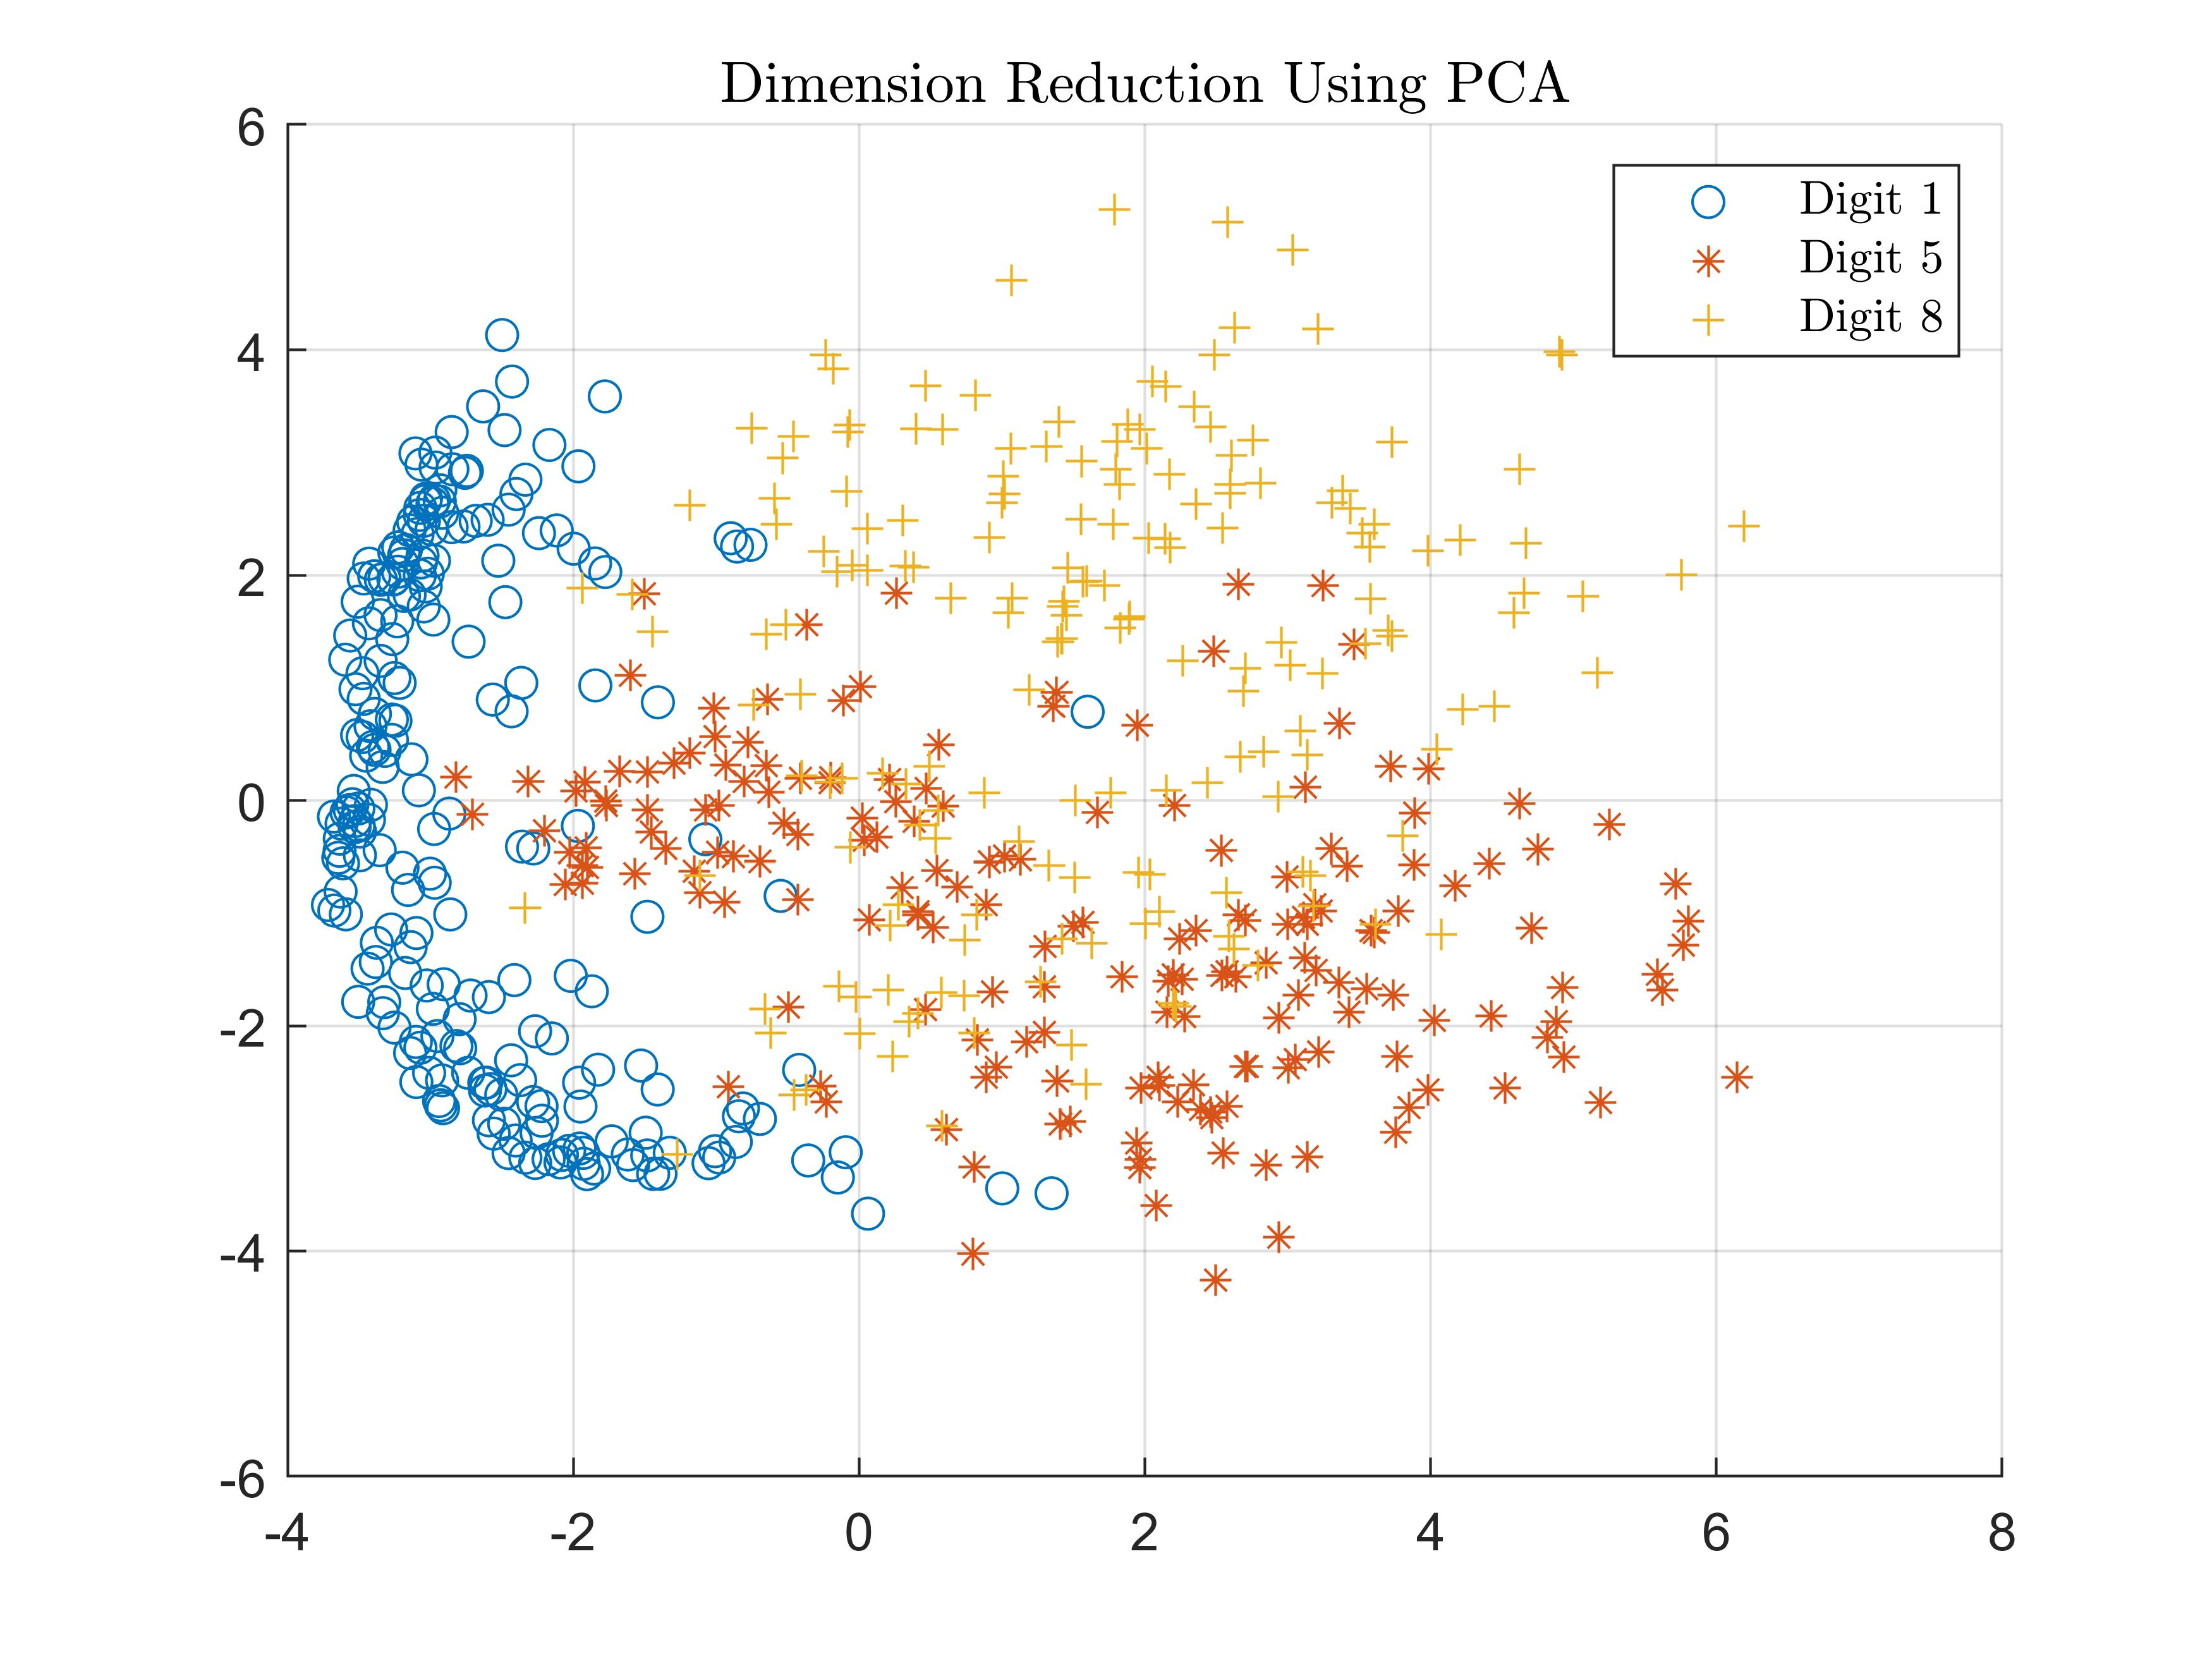
\includegraphics[width=0.9\textwidth]{PCA.jpg}
	\caption{Dimension Reduction Using PCA}
	\label{fig:1}
\end{figure}

\hspace{0.7cm}
Observing this result plot, we can find that the data points of digit 1 distribute on the left side, while digit 5 lies on the bottom-right, digit 8 on the top-right. We can see that the PCA process does separate those datapoints in the 2-dimension plot.

\hspace{0.7cm}
Next, we do clustering to divide the data points to 3 clusters. We firstly try to use K-means clustering, an unsupervised learning algorithm that divide unlabelled dataset into $k$ different clusters. It is a centroid-based clustering method, which will choose a set of $k$ centroids and keep updating to make the final result converge. Here I use the build-in function in MATLAB \texttt{kmeans()} to adopt clustering after PCA. The codes are shown as following and the clustering result is shown in Figure \ref{fig:2}.

\begin{footnotesize}
\begin{minted}[mathescape,breaklines,breakindent=0em,linenos,numbersep=5pt,gobble=0,framesep=2mm]{matlab}
% ----- K-Means Clustering -----
[idx,C] = kmeans(score, 3);
x1 = min(score(:, 1)):0.01:max(score(:, 1));
x2 = min(score(:, 2)):0.01:max(score(:, 2));
[x1G,x2G] = meshgrid(x1, x2);
XGrid = [x1G(:), x2G(:)];
idx2Region = kmeans(XGrid, 3, 'MaxIter', 40, 'Start', C);
% ------------------------------
\end{minted}
\end{footnotesize}

\begin{figure}[!htbp]
	\centering
	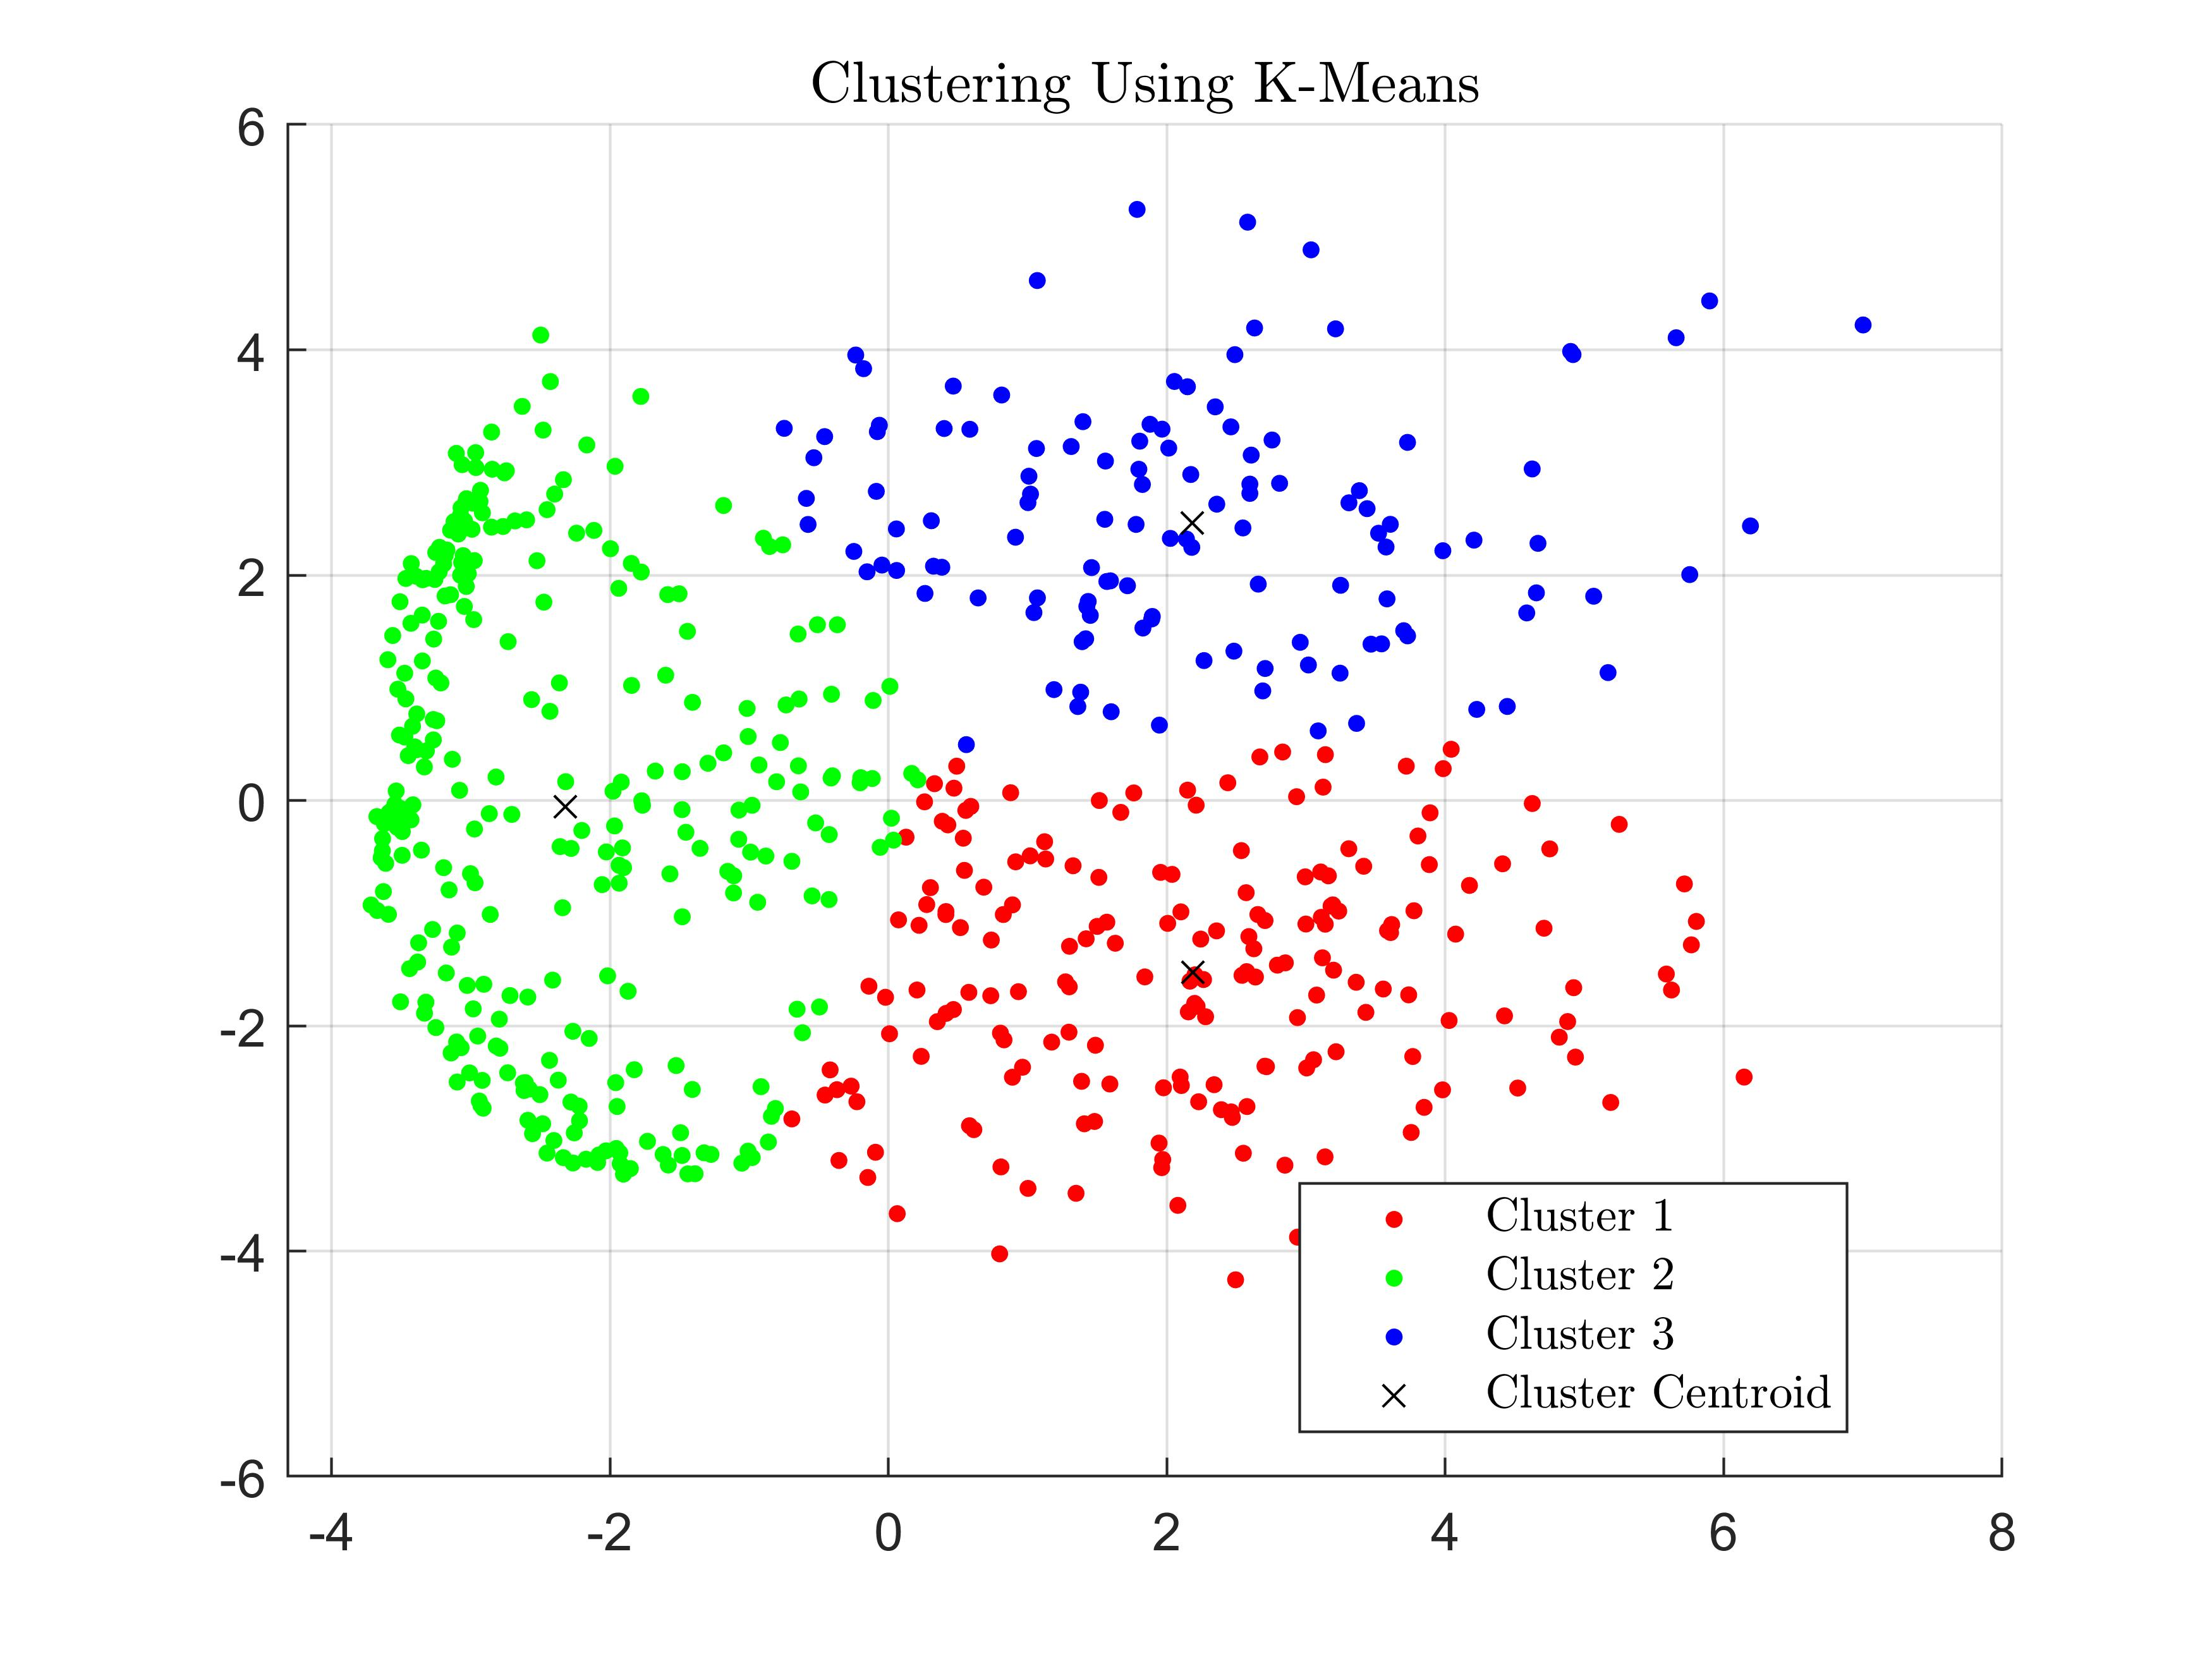
\includegraphics[width=0.9\textwidth]{KMEANS.jpg}
	\caption{Clustering Result Using K-means after PCA}
	\label{fig:2}
\end{figure}


\hspace{0.7cm}
In Figure \ref{fig:2}, I also mark the centroid of every cluster on the plot. We can observe that the clustering result fits our intuition: the 3 clusters are roughly digit 1, digit 5, digit 8. And as is obviously shown, the similar data points are clustered together, marked with the same color.



\hspace{0.7cm}
Here I also try hierarchical clustering, a connectively-based clustering method. Different from the centroid-based clustering method K-means, hierarchical clustering will try to calculate the distances between clusters and make a final decision. Here I use average linkage, where the distances between different clusters are determined by the average value of the distances between every data pairs. In mathematical language, distance between cluster $r$ and $s$ $L(r,s)$ is calculated by Equation 4.
\begin{equation}
	L\left( r,s \right) =\frac{1}{n_rn_s}\sum_{i=1}^{n_r}{\sum_{j=1}^{n_s}{D\left( x_{ri},x_{sj} \right)}}
\end{equation}

\hspace{0.7cm}
I adopt hierarchical clustering by \texttt{linkage()} and \texttt{cluster()} method, here as the following shows the codes related to hierarchical clustering. The dendrogram plot is shown in Figure \ref{fig:3} and the result is shown in Figure \ref{fig:4}.

\begin{footnotesize}
\begin{minted}[mathescape,breaklines,breakindent=0em,linenos,numbersep=5pt,gobble=0,framesep=2mm]{matlab}
% ----- Hierarchical Clustering -----
%create the linkage tree using average-link
Z = linkage(score(:,1:2),'average','euclidean'); 
c = cluster(Z,'maxclust',3);
% -----------------------------------
\end{minted}
\end{footnotesize}

\begin{figure}[!htbp]
	\centering
	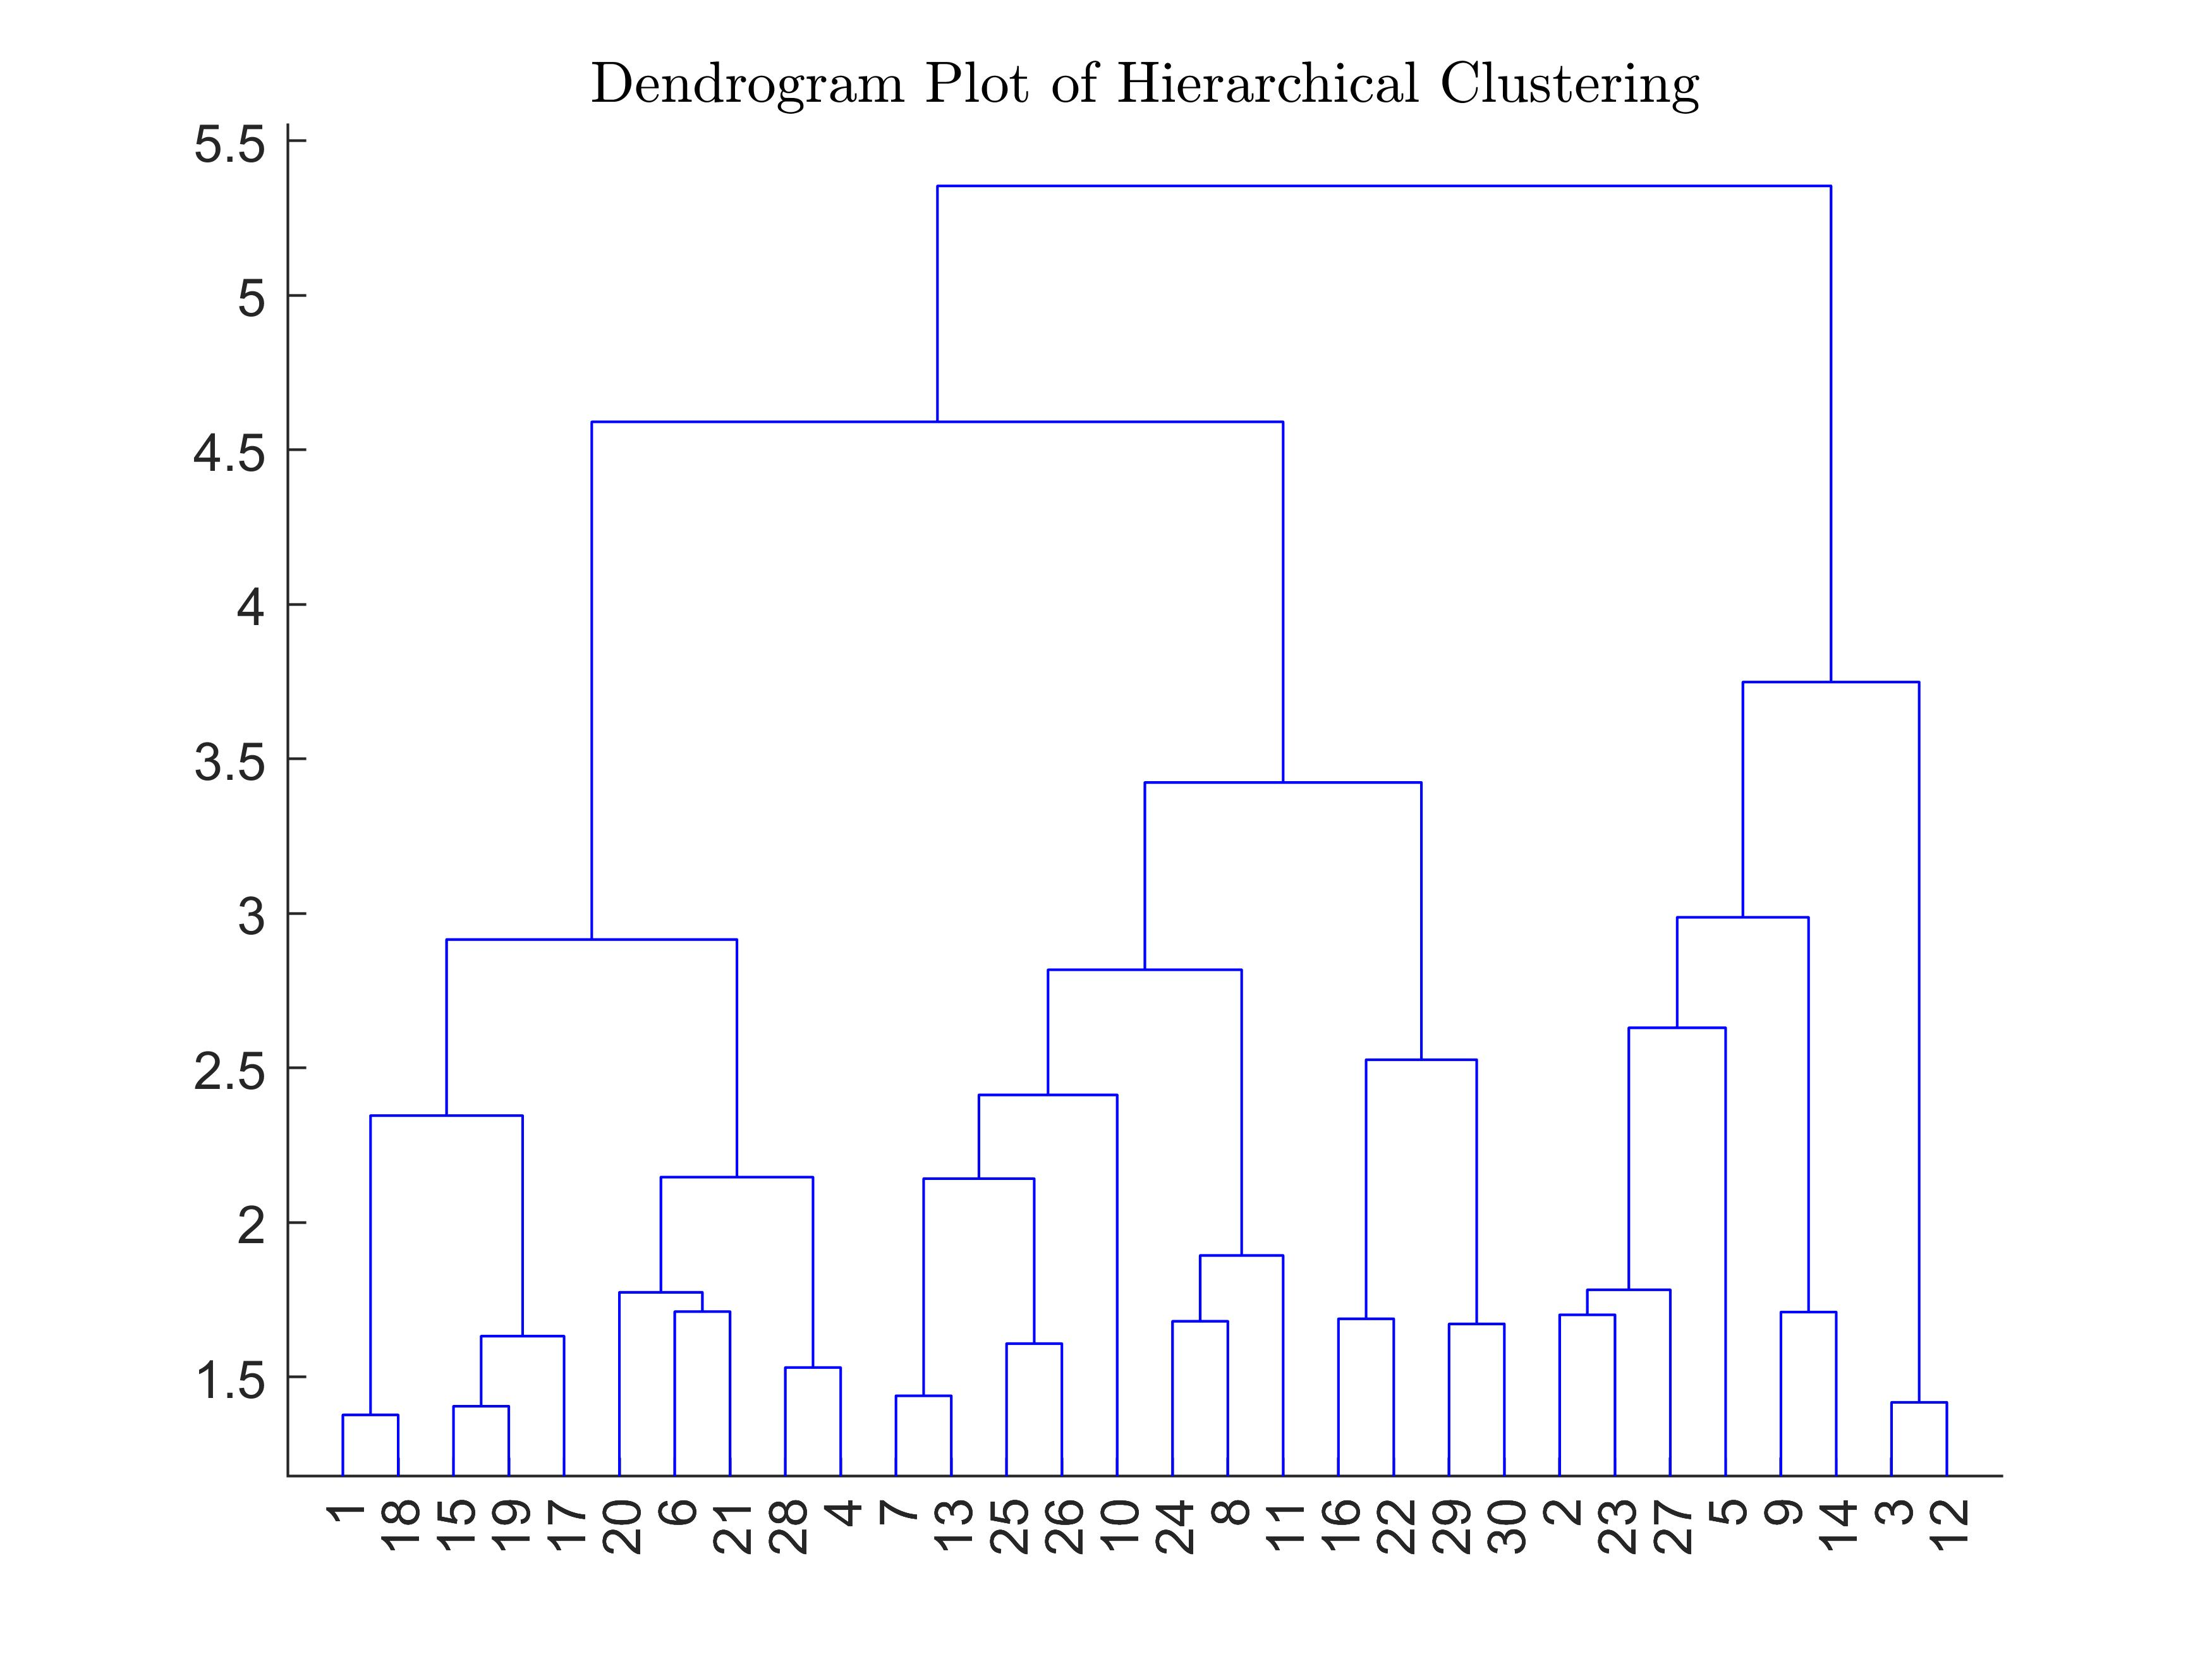
\includegraphics[width=0.9\textwidth]{DEN.jpg}
	\caption{Dendrogram Plot of Hiererachical Clustering after PCA}
	\label{fig:3}
\end{figure}

\begin{figure}[!htbp]
	\centering
	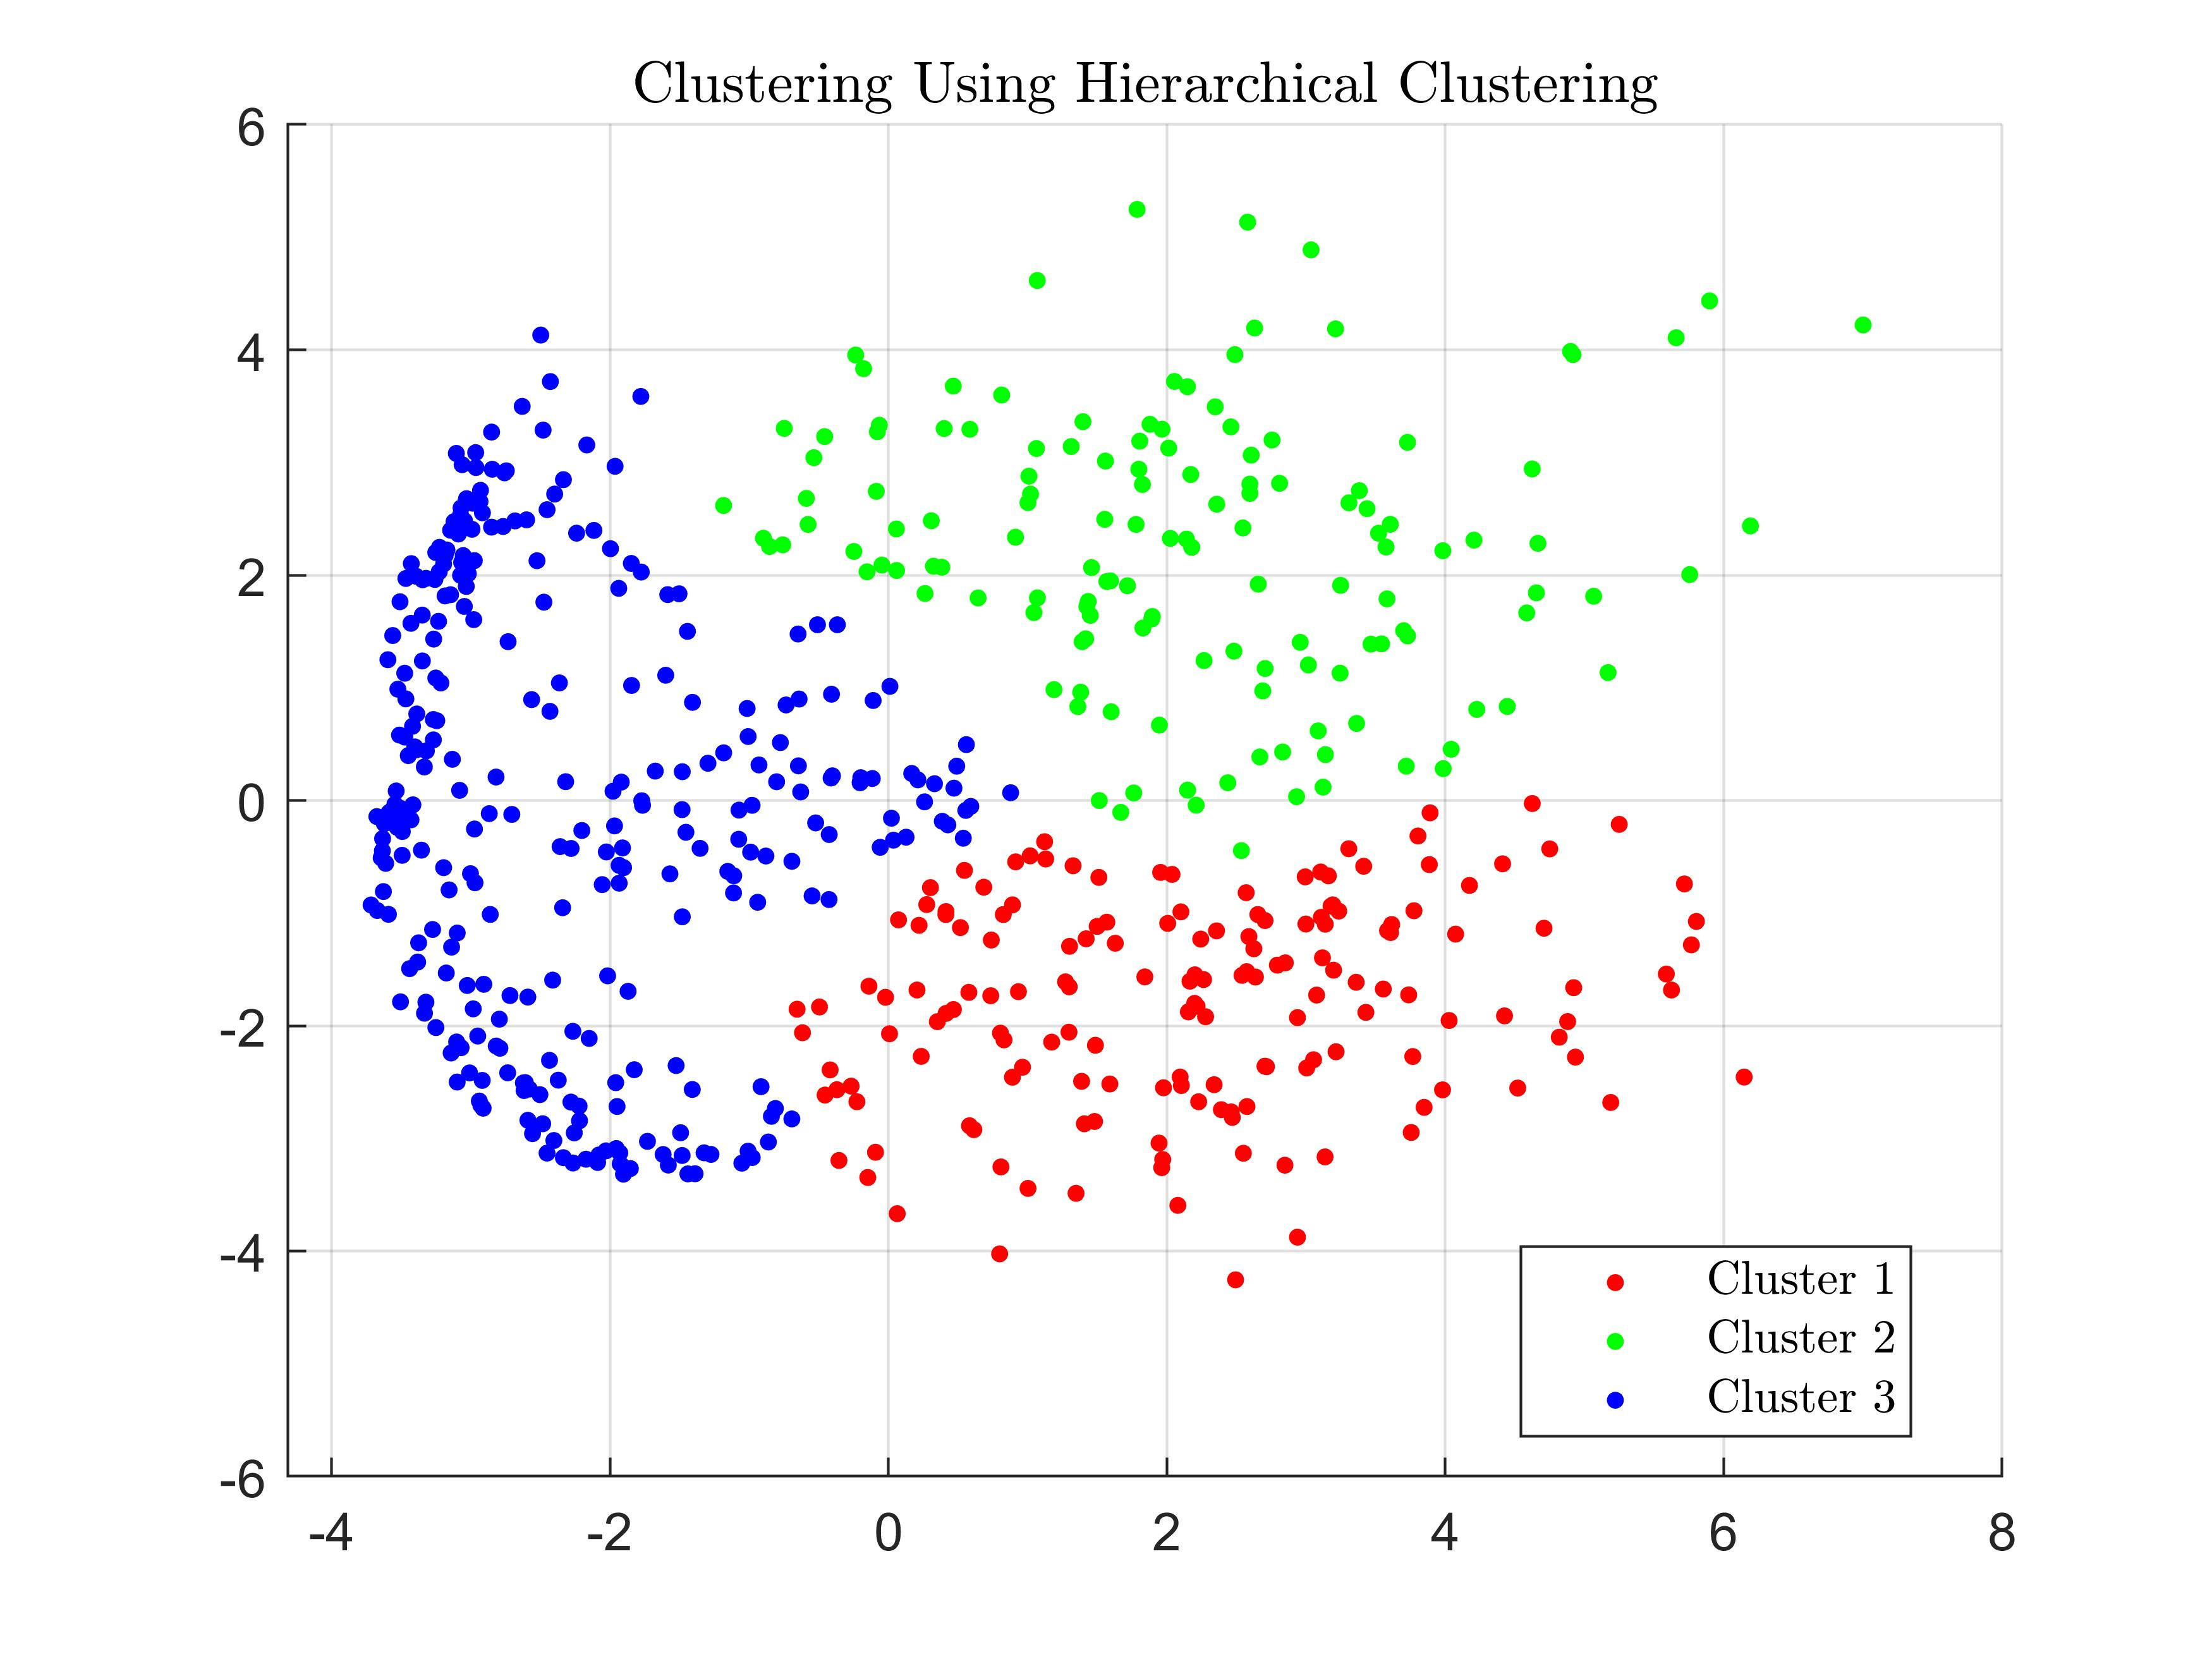
\includegraphics[width=0.9\textwidth]{HIERACHICAL.jpg}
	\caption{Clustering Result Using Hierarchical Clustering after PCA}
	\label{fig:4}
\end{figure}

\hspace{0.7cm}
Gaussian mixture model (GMM) clustering, a distribution based clustering method, is also adopted to complete the clustering task. As our options of covariance matrix type change, the clustering result also changes. Here as the following shows the codes related to GMM clustering. The result is shown in Figure \ref{fig:5}.

\begin{footnotesize}
\begin{minted}[mathescape,breaklines,breakindent=0em,linenos,numbersep=5pt,gobble=0,framesep=2mm]{matlab}
% ----------------- GMM clustering -----------------
k = 3; % Number of GMM components
options = statset('MaxIter',1000);

% Options for covariance matrix type
Sigma = {'diagonal','full'}; 
nSigma = numel(Sigma);

% Indicator for identical or nonidentical covariance matrices
SharedCovariance = {true,false}; 
SCtext = {'true','false'};
nSC = numel(SharedCovariance);

d = 500; % Grid length
x1 = linspace(min(score(:,1))-2, max(score(:,1))+2, d);
x2 = linspace(min(score(:,2))-2, max(score(:,2))+2, d);
[x1grid,x2grid] = meshgrid(x1,x2);
X0 = [x1grid(:) x2grid(:)];

threshold = sqrt(chi2inv(0.99,2));
count = 1;
for i = 1:nSigma
    for j = 1:nSC
        gmfit = fitgmdist(score,k,'CovarianceType',Sigma{i}, ...
            'SharedCovariance',SharedCovariance{j},'Options',options); % Fitted GMM
        clusterX = cluster(gmfit,score); % Cluster index 
        mahalDist = mahal(gmfit,X0); % Distance from each grid point to each GMM component
        % Draw ellipsoids over each GMM component and show clustering result.
        subplot(2,2,count);
        h1 = gscatter(score(:,1),score(:,2),clusterX);
        hold on
            for m = 1:k
                idx = mahalDist(:,m)<=threshold;
                Color = h1(m).Color*0.75 - 0.5*(h1(m).Color - 1);
                h2 = plot(X0(idx,1),X0(idx,2),'.','Color',Color,'MarkerSize',1);
                uistack(h2,'bottom');
            end    
        plot(gmfit.mu(:,1),gmfit.mu(:,2),'kx','LineWidth',2,'MarkerSize',10)
        title(sprintf('Sigma is %s\nSharedCovariance = %s',Sigma{i},SCtext{j}),'FontSize',8)
        legend(h1,{'1','2','3'})
        hold off
        count = count + 1;
    end
end
% --------------------------------------------
\end{minted}
\end{footnotesize}

\begin{figure}[!htbp]
	\centering
	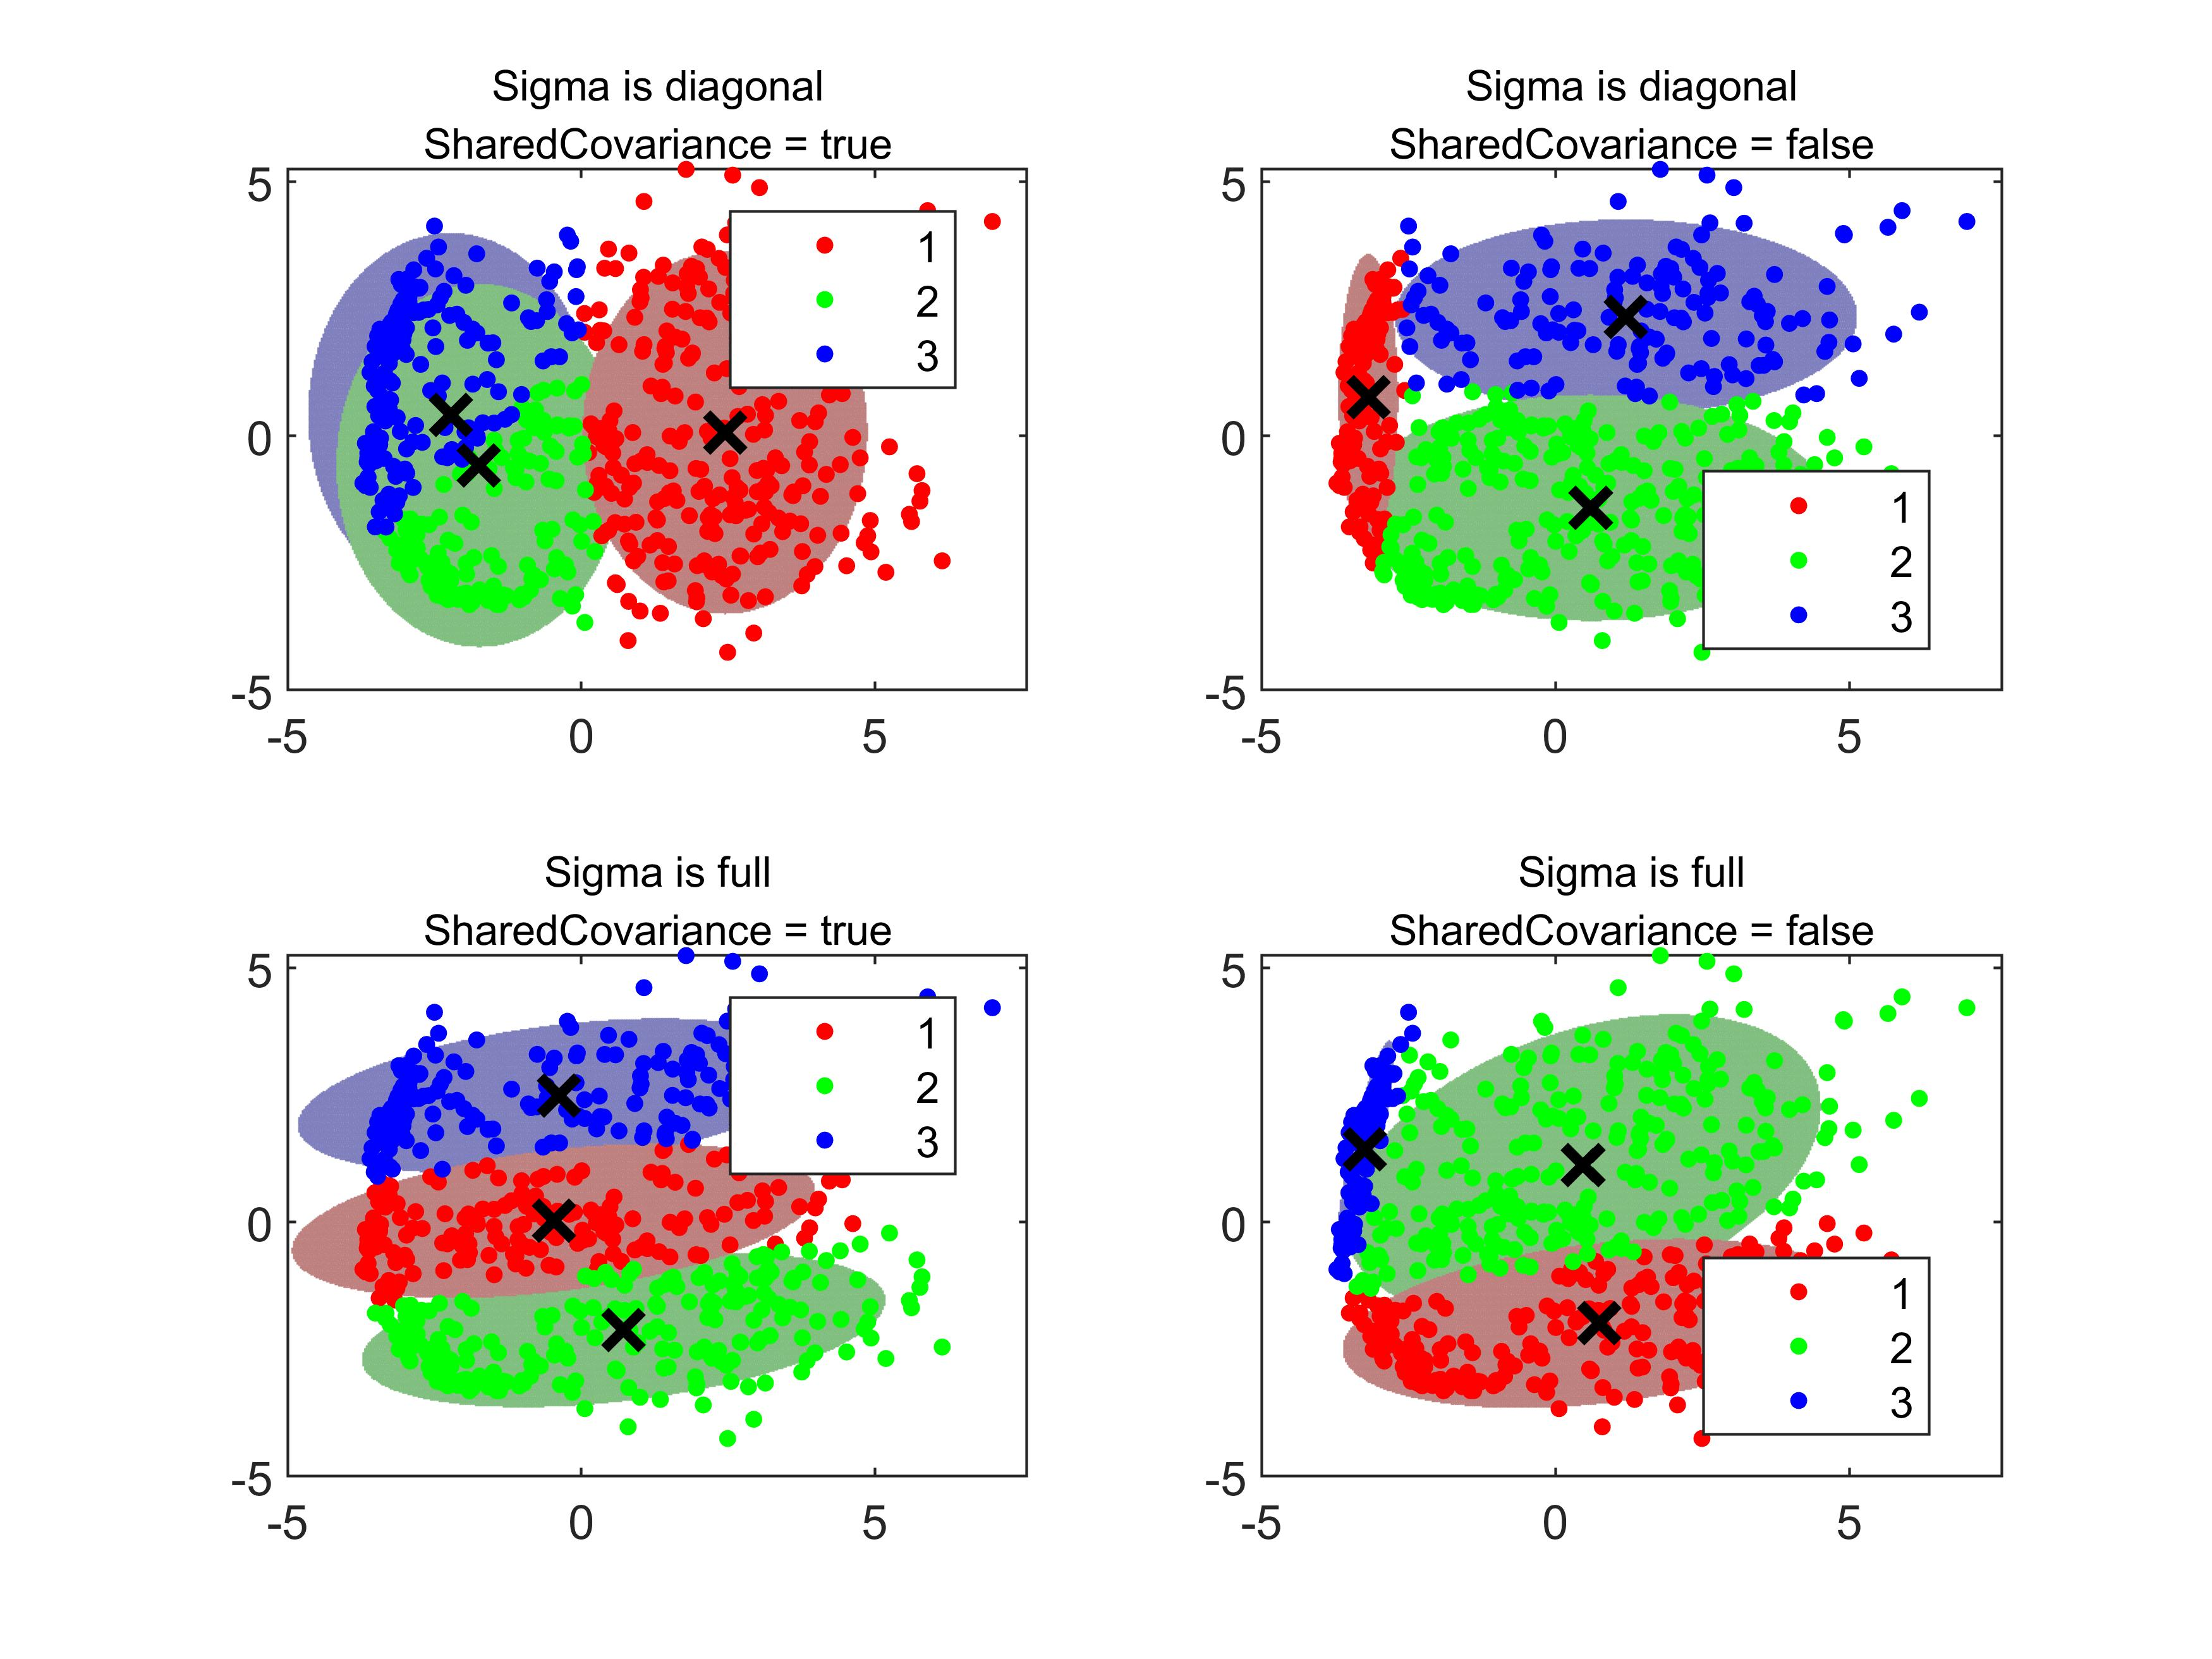
\includegraphics[width=0.9\textwidth]{GMM.jpg}
	\caption{Clustering Result Using GMM Clustering After PCA}
	\label{fig:5}
\end{figure}

\subsection{Linear Discriminant Analysis (LDA) and Clustering}
\hspace{0.7cm}
Linear discriminant analysis is a dimensionality reduction technique that is commonly used for supervised classification problems. PCA is used to maximize the variance of the projected data, while it may lead our data impossible to divide. Different with that, LDA finds most discriminant projection by maximizing between-class distance and minimizing within-class distance.
In this part, I use LDA to reduce dimensions of the same partial MNIST dataset containing only digit 1,5,8, followed by adopting different clustering methods.

\hspace{0.7cm}
At first, we still need to pre-process the data matrix by deleting the mean value in each column. Then the between-class scatter $S_b$ can be calculated by Equation 5, while within-class scatter $S_w$ can be calculated by Equation 6, where $S_1, S_2, S_3$ are the covariance matrix of data from digit 1, 5, 8.
\begin{equation}
	S_b=\sum_{k=1}^K{N_k}\left( m_k-m \right) \left( m_k-m \right) ^T
\end{equation}
\begin{equation}
	S_w=S_1+S_2+S_3
\end{equation}

\hspace{0.7cm}
The trace of those 2 matrices represent the between-class distance and the within-class distance. To maximize between-class distance and minimize within-class distance, we need to find the parameters that satisfies the following expression.
\begin{equation*}
	\underset{w}{\mathrm{arg}\max}\frac{trace\left( W^TS_bW \right)}{trace\left( W^TS_wW \right)}
\end{equation*}

\hspace{0.7cm}
Therefore, the optimal transformation is given by solving a generalized eigenvalue problem for $S_w^{-1}S_b$. To be noteworthy, the within-class scatter is singular for most of the cases, here we add an identity part $kI$ with $k=1e-10$ to $S_w$, making it has full rank. Finally we take the leading 2 eigenvectors as our projection directions to reduce the dimension from $784$ to $2$.

\hspace{0.7cm}
The whole implementation in MATLAB is given as following. The LDA result is shown in Figure \ref{fig:6}.
\begin{footnotesize}
\begin{minted}[mathescape,breaklines,breakindent=0em,linenos,numbersep=5pt,gobble=0,framesep=2mm]{matlab}
images = images.';
class1 = images(labels==1,:);
class5 = images(labels==5,:);
class8 = images(labels==8,:);

% class means
m1 = mean(class1);
m5 = mean(class5);
m8 = mean(class8);
m = mean(images);
% class covariance matrix
s1 = cov(class1);
s5 = cov(class5);
s8 = cov(class8);
% within class scatter matrix
sw = s1 + s5 + s8;

% between class scatter matrix
mb = zeros(3, 784);
mb(1, :) =  m1 - m;
mb(2, :) =  m5 - m;
mb(3, :) =  m8 - m;
sb = mb.' * mb;

% computing the LDA projection vector
[v, d] = eigs((inv(sw + 1e-10 * eye(784))) * sb);

% computing the projection score:
score = images * v(:, 1:2);
\end{minted}
\end{footnotesize}

\begin{figure}[!htbp]
	\centering
	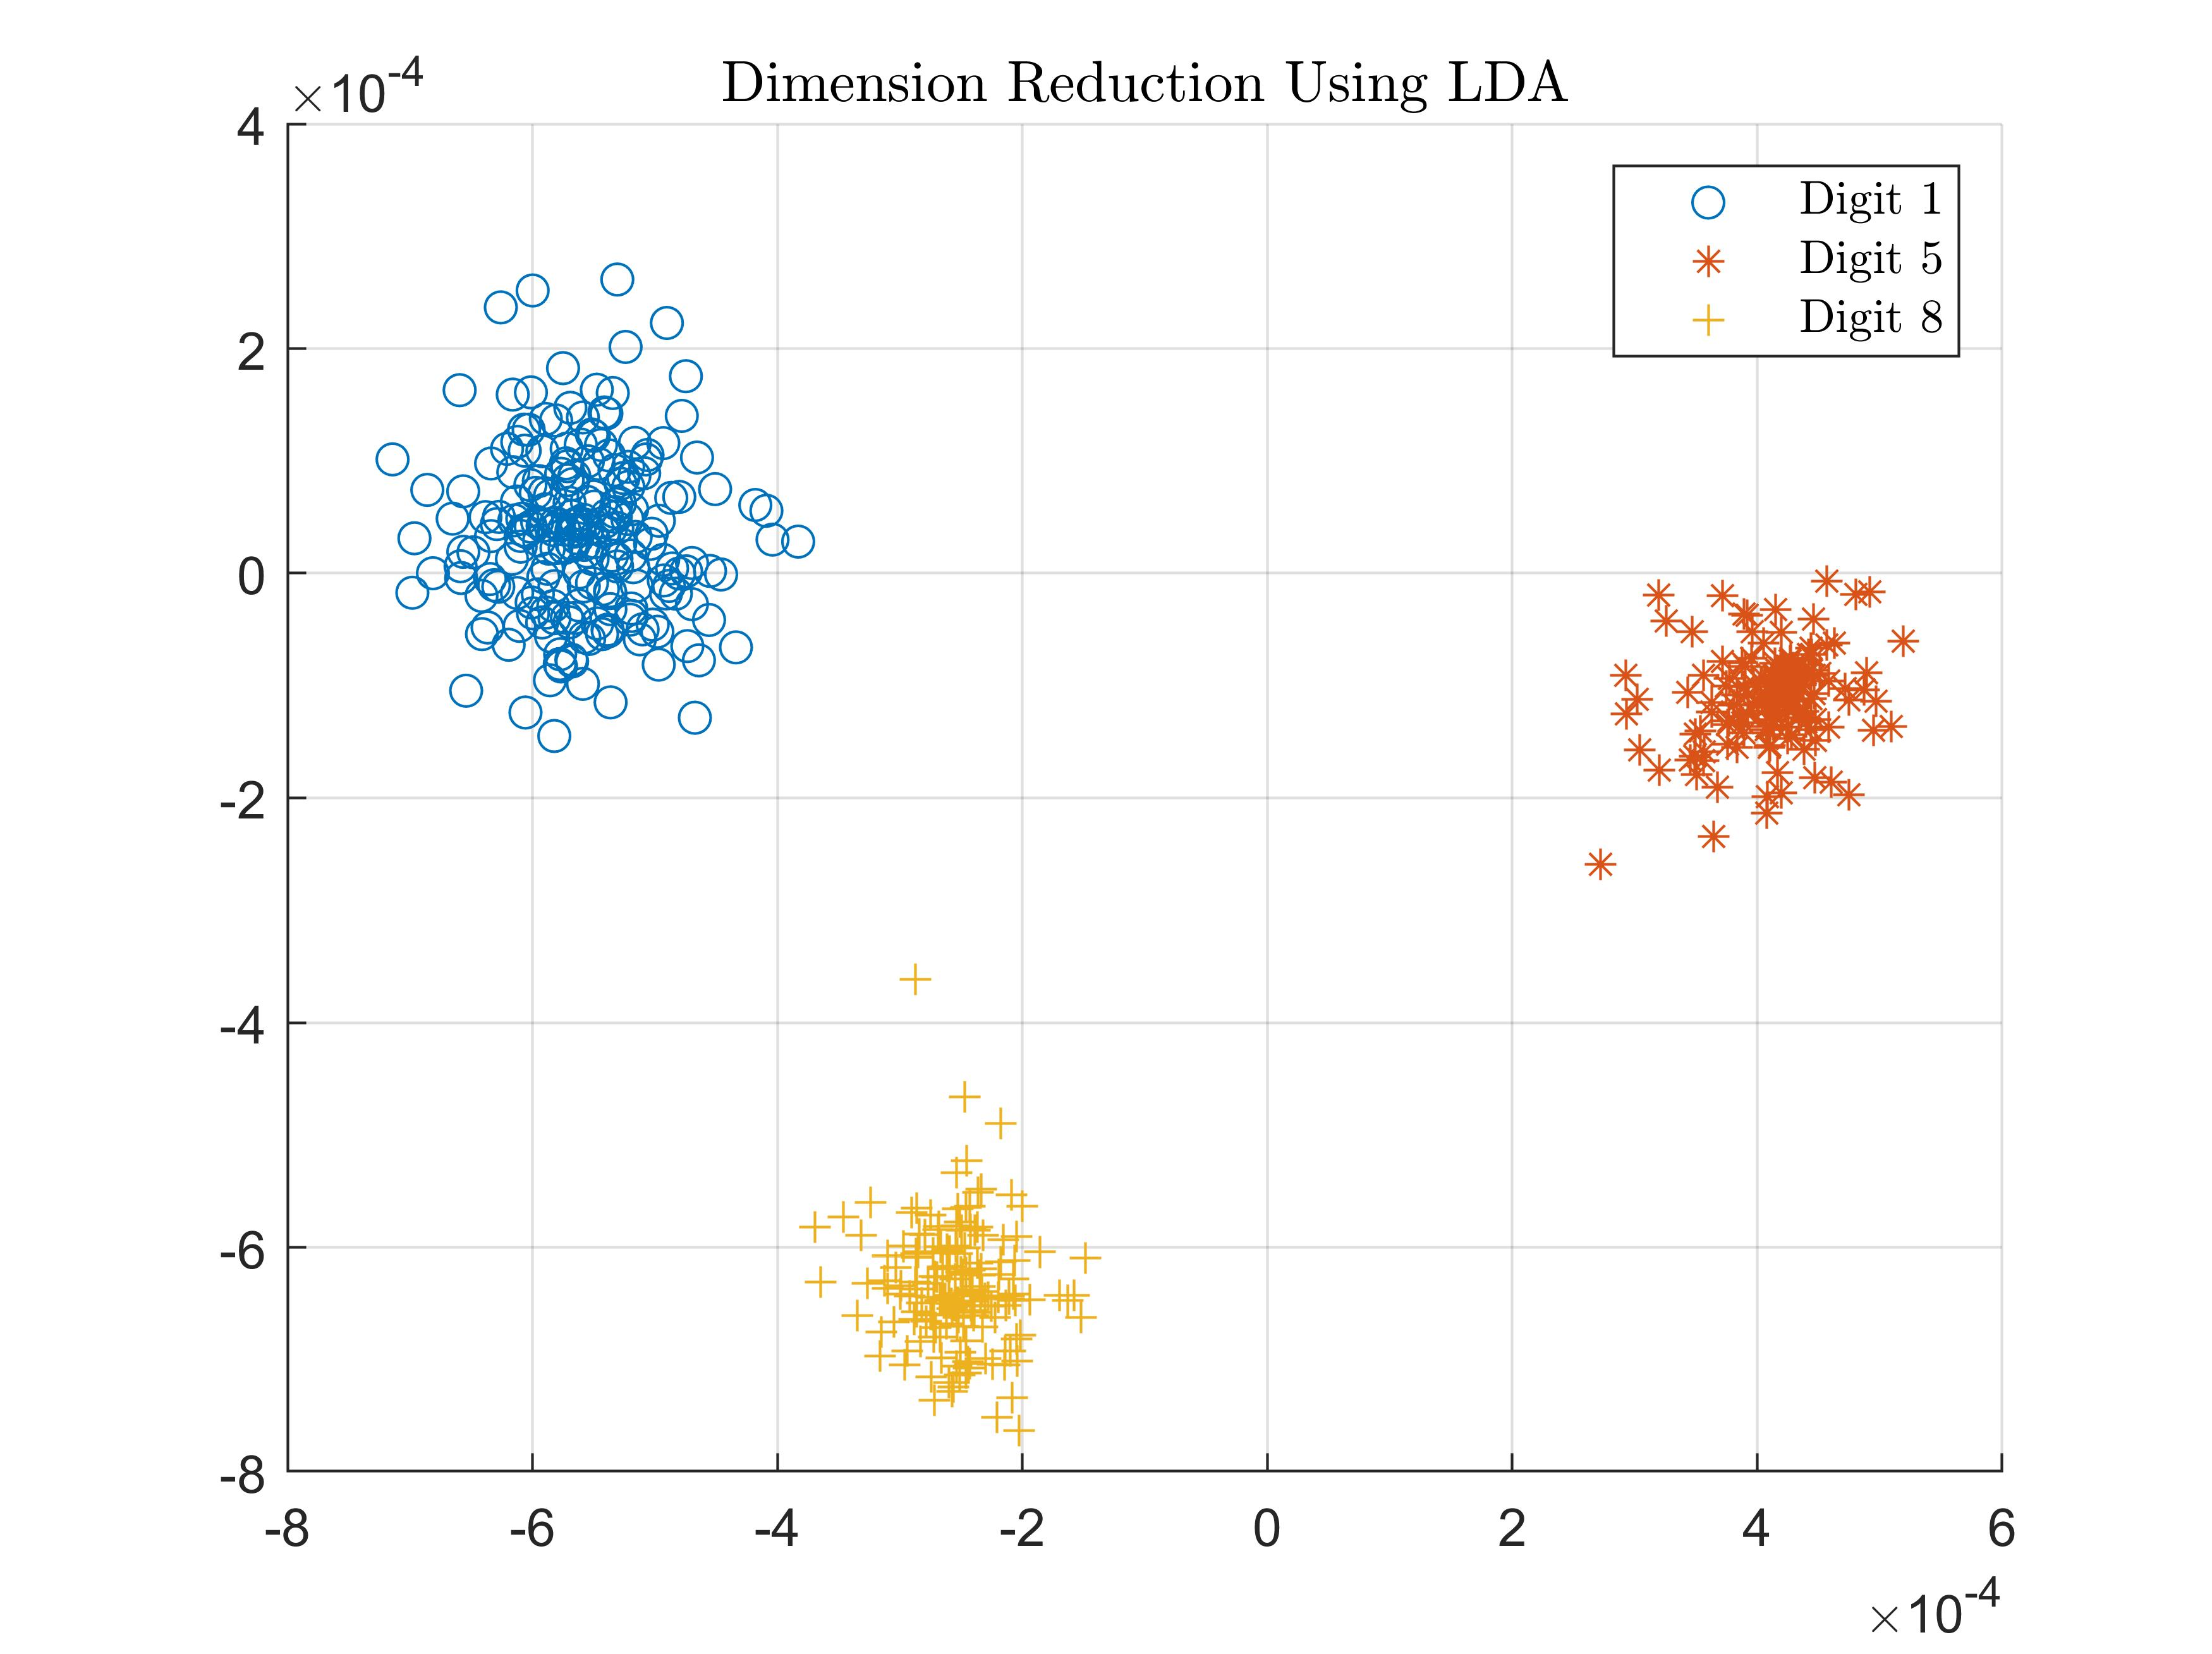
\includegraphics[width=0.9\textwidth]{LDA.jpg}
	\caption{Dimension Reduction Using LDA}
	\label{fig:6}
\end{figure}

\hspace{0.7cm}
From the result, we can clearly seen that the different digits are divided into different clusters in the 2-D plot, with no overlapping area. Then we repeat the clustering process introduced in PCA part, The results are shown in Figure \ref{fig:7}, \ref{fig:8}, \ref{fig:9}.

\begin{figure}[!htbp]
	\centering
	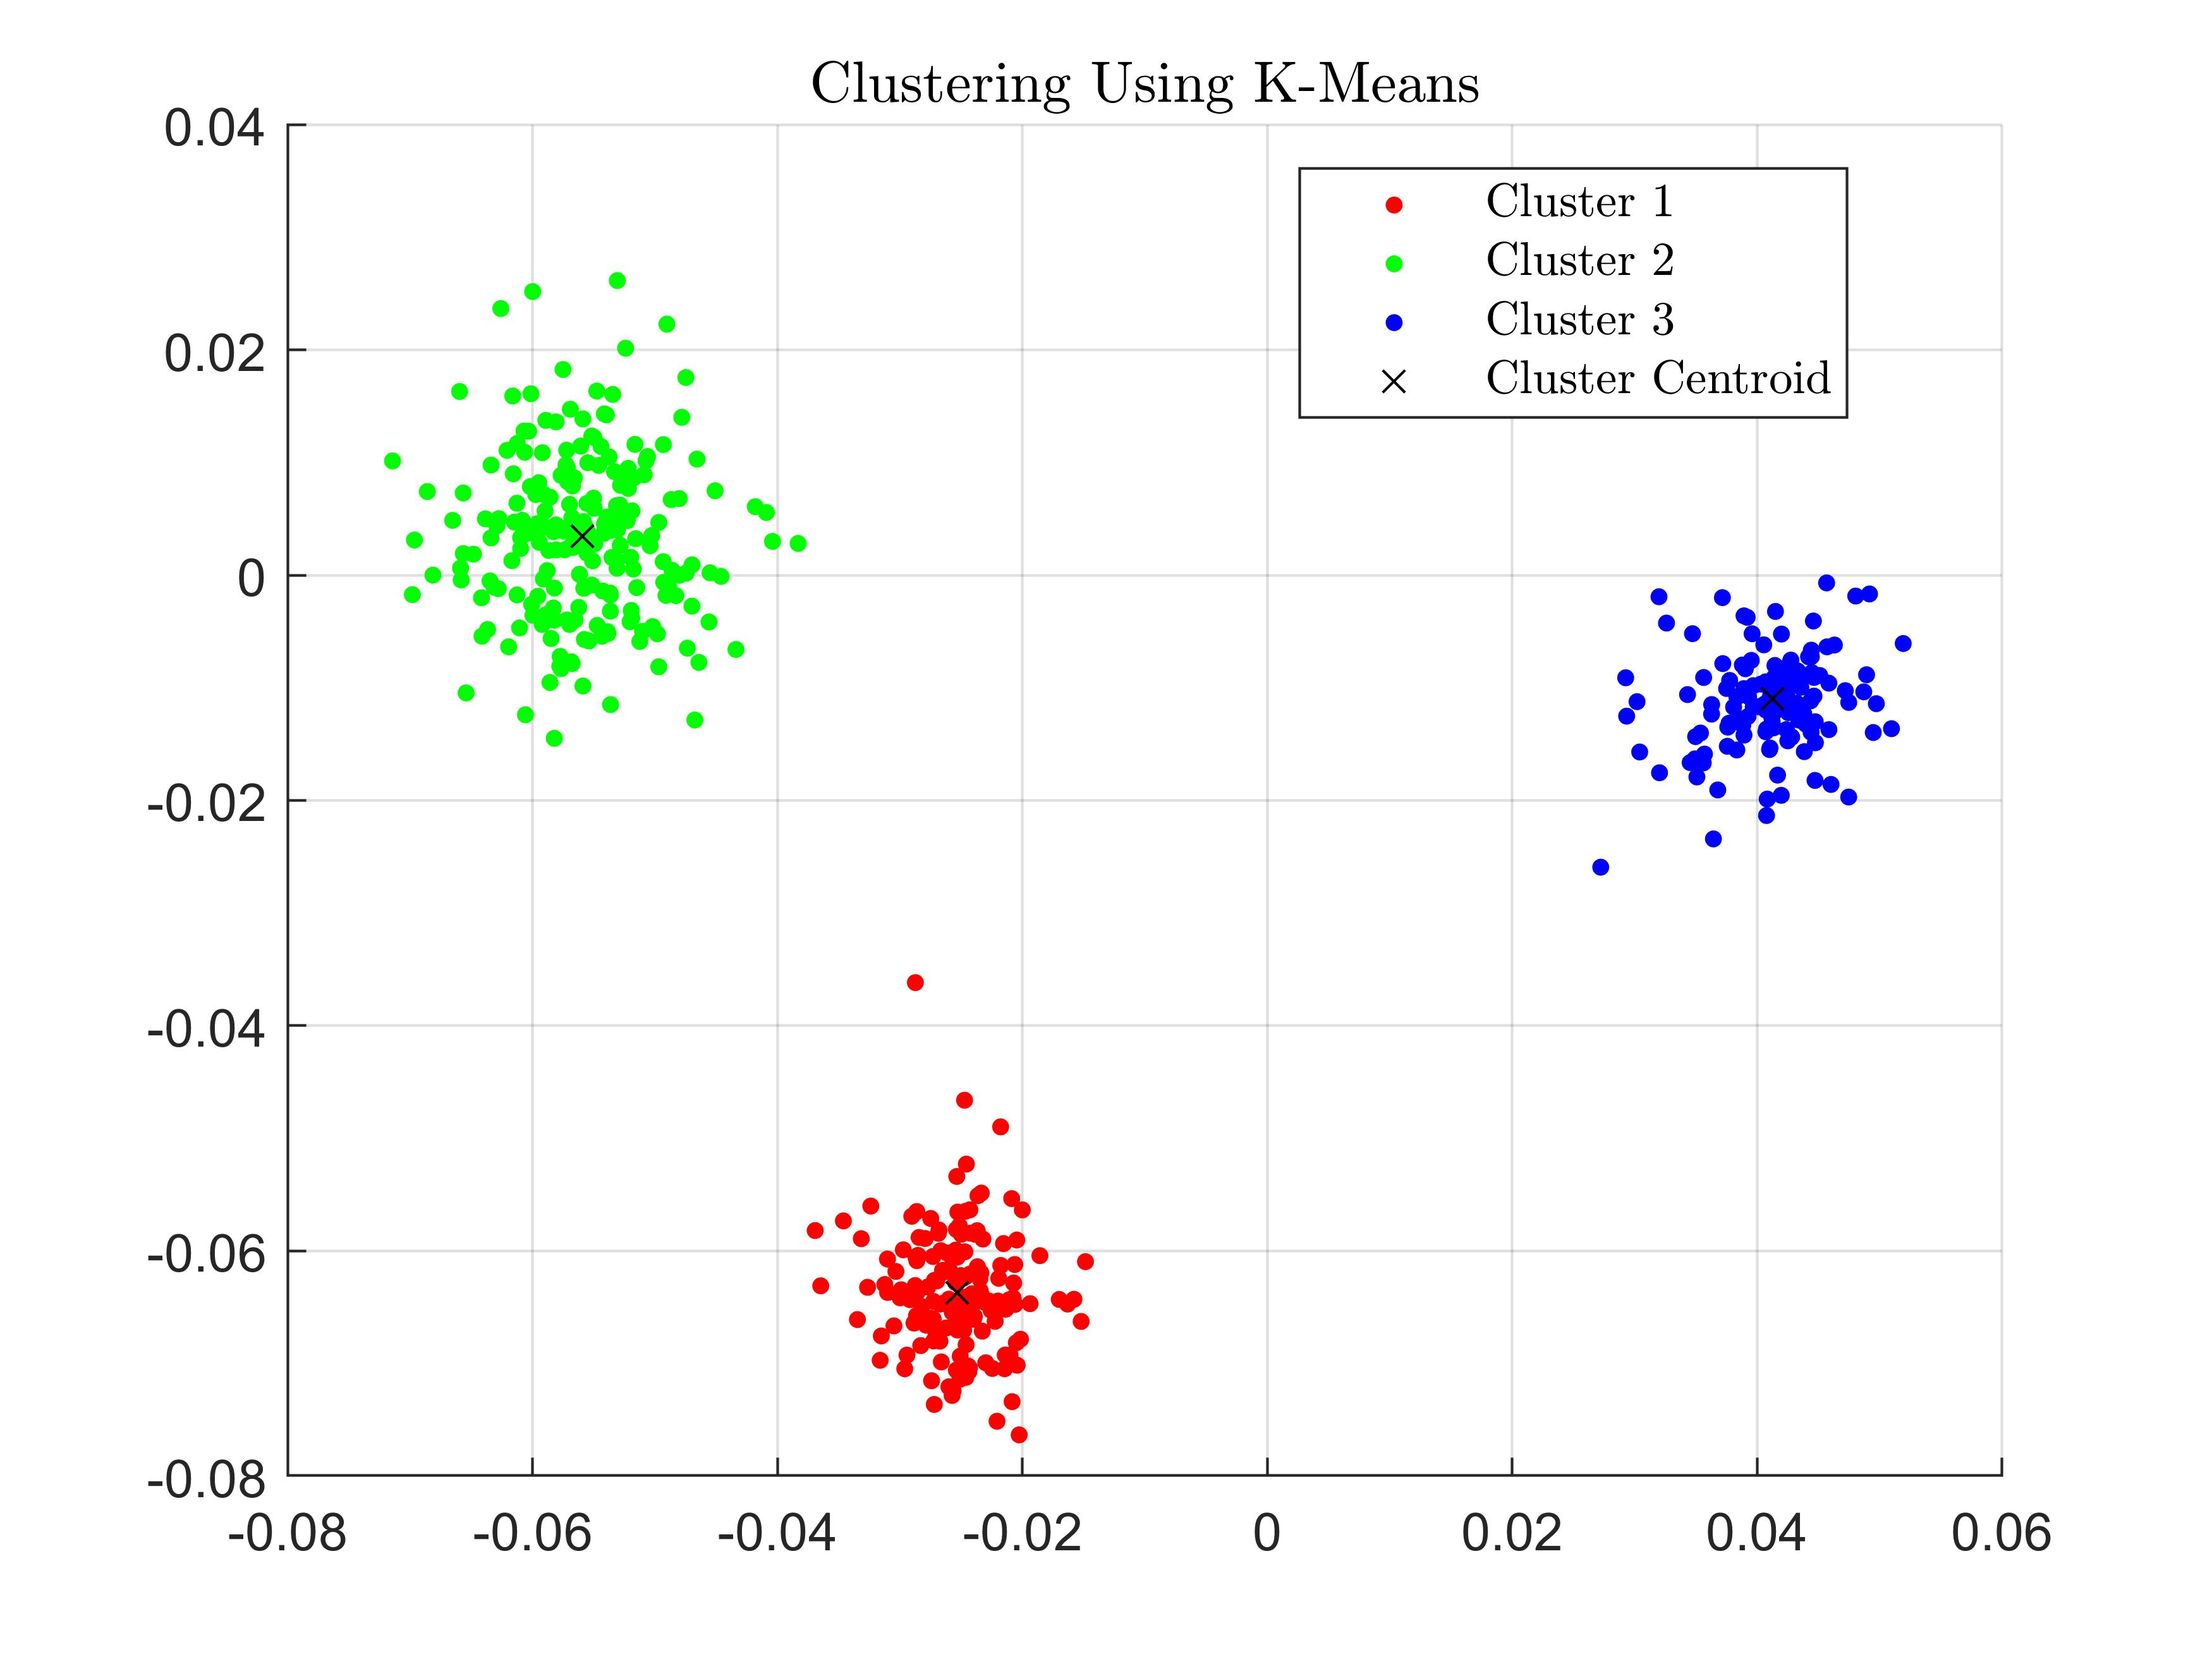
\includegraphics[width=0.9\textwidth]{KMEANS2.jpg}
	\caption{Clustering Result Using K-means after LDA}
	\label{fig:7}
\end{figure}

\begin{figure}[!htbp]
	\centering
	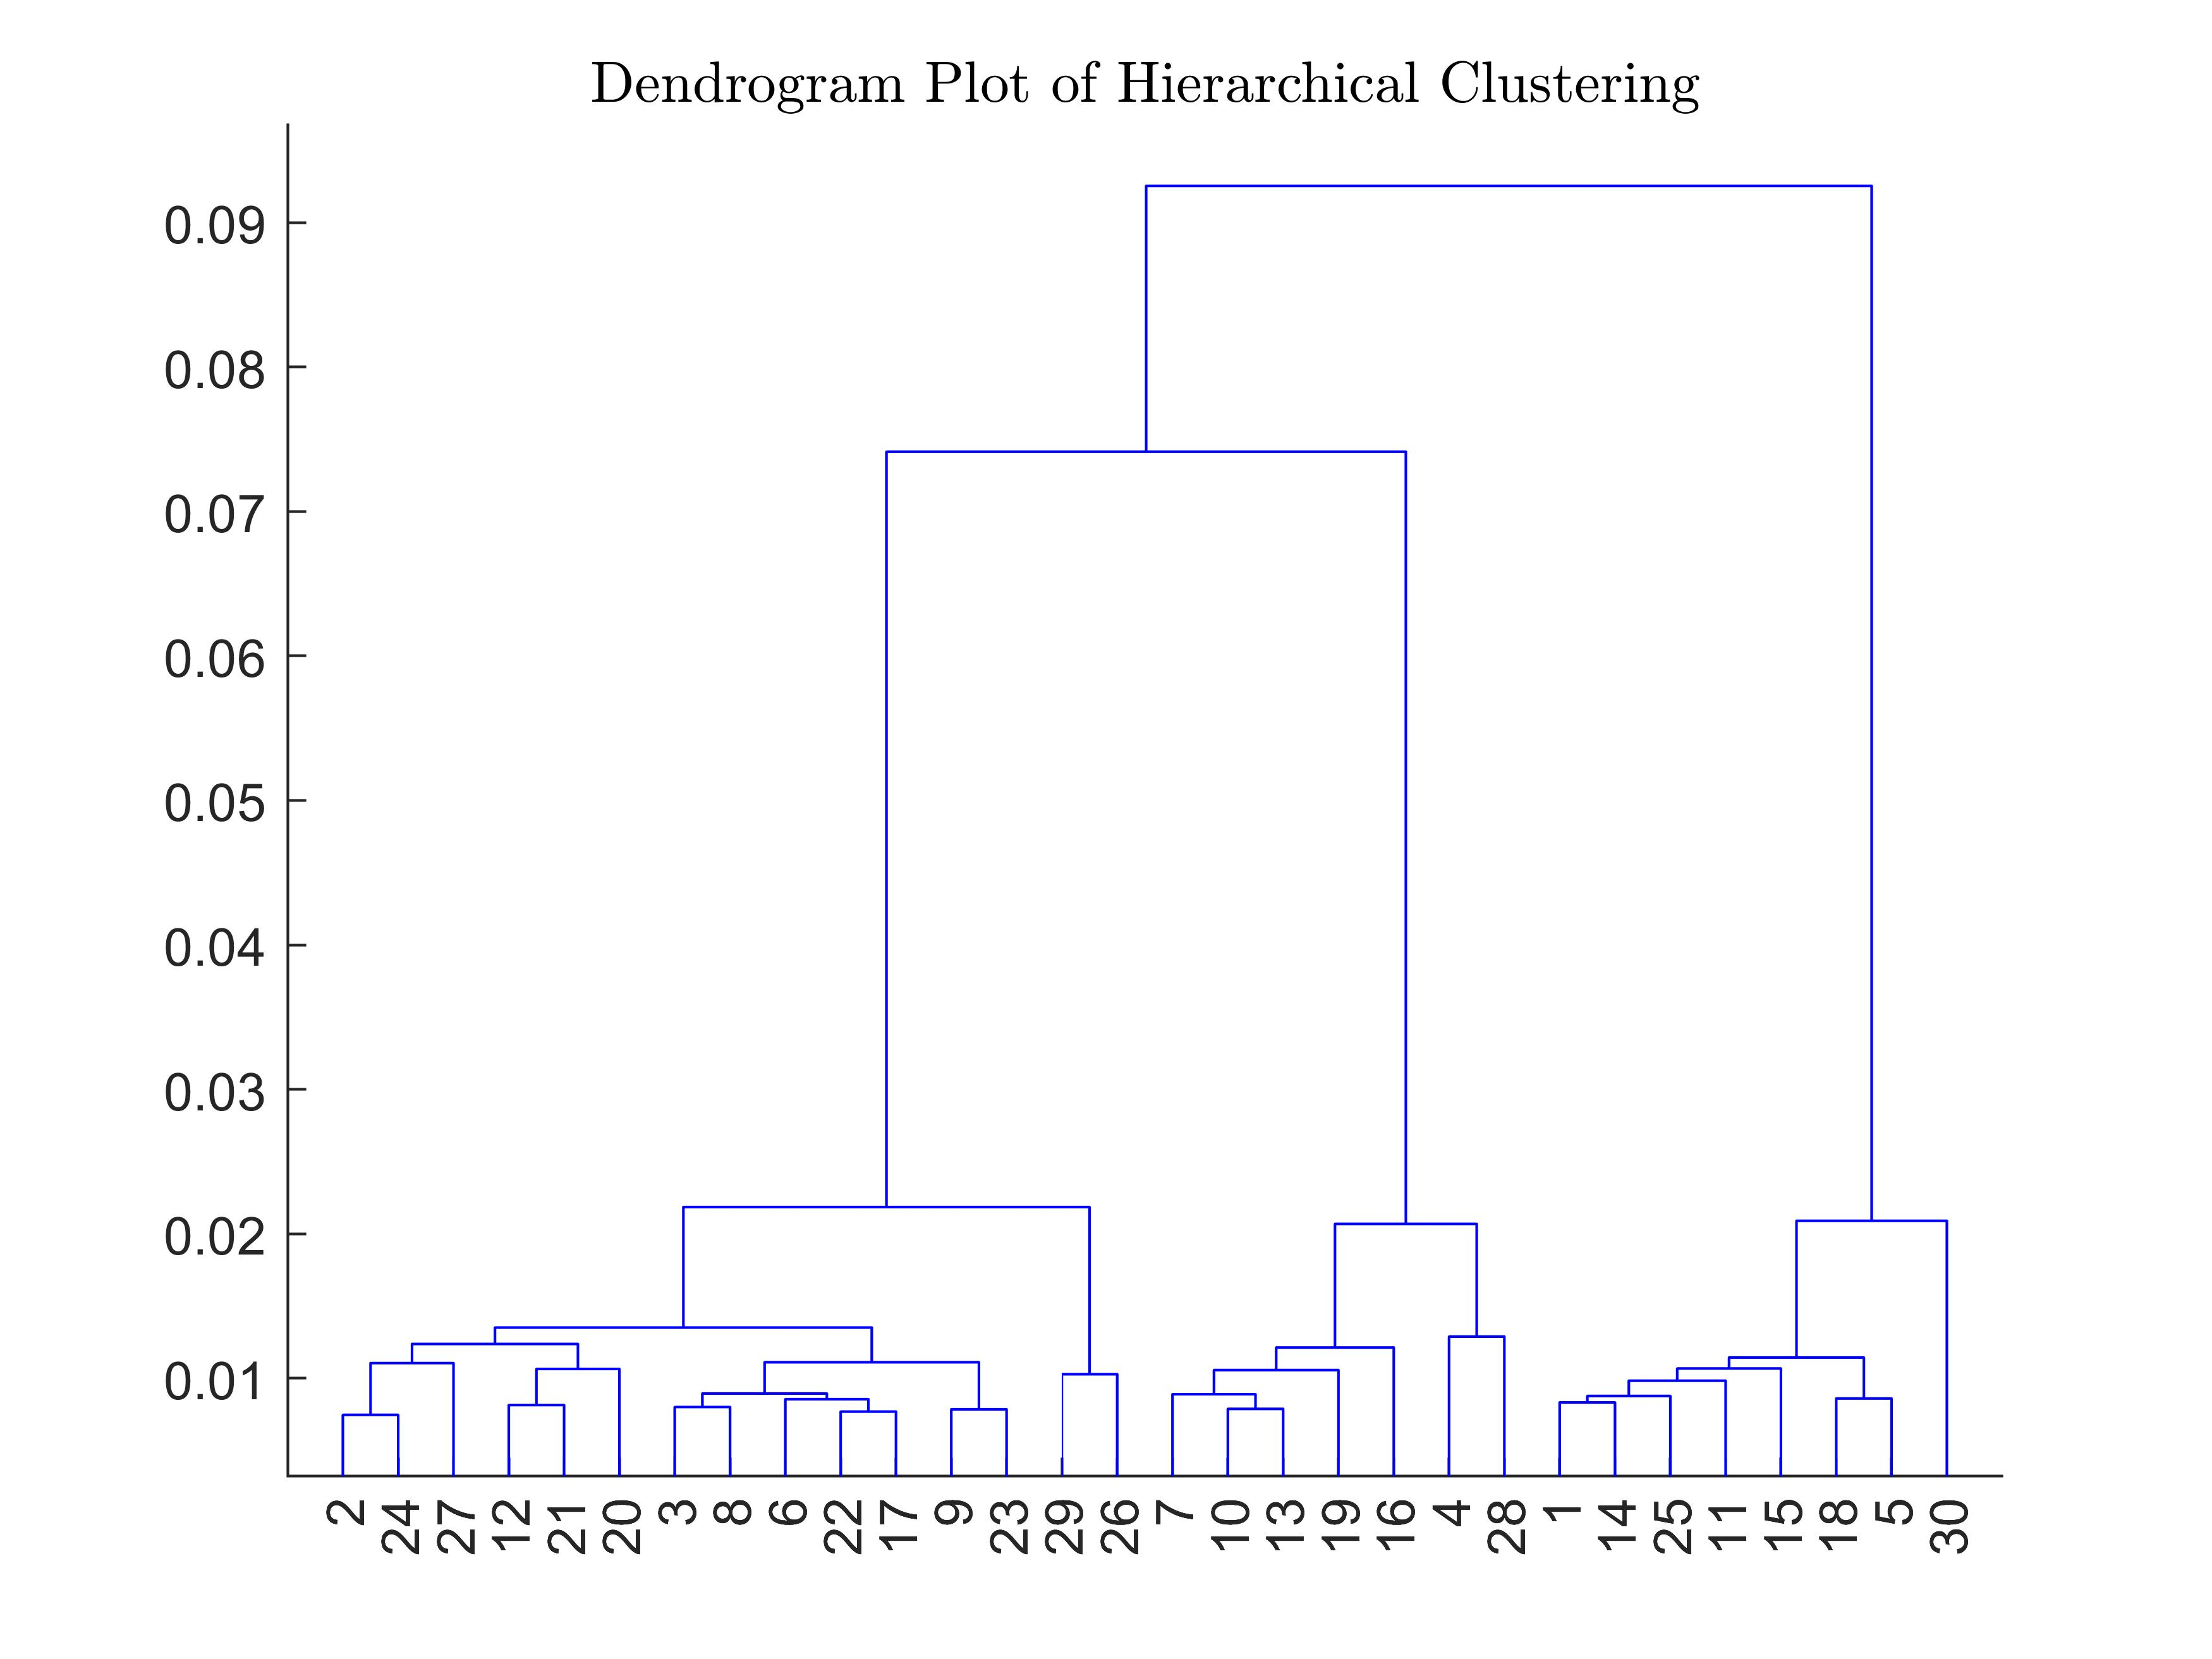
\includegraphics[width=0.9\textwidth]{DEN2.jpg}
	\caption{Dendrogram Plot of Hierarchical Clustering after LDA}
	\label{fig:8}
\end{figure}

\begin{figure}[!htbp]
	\centering
	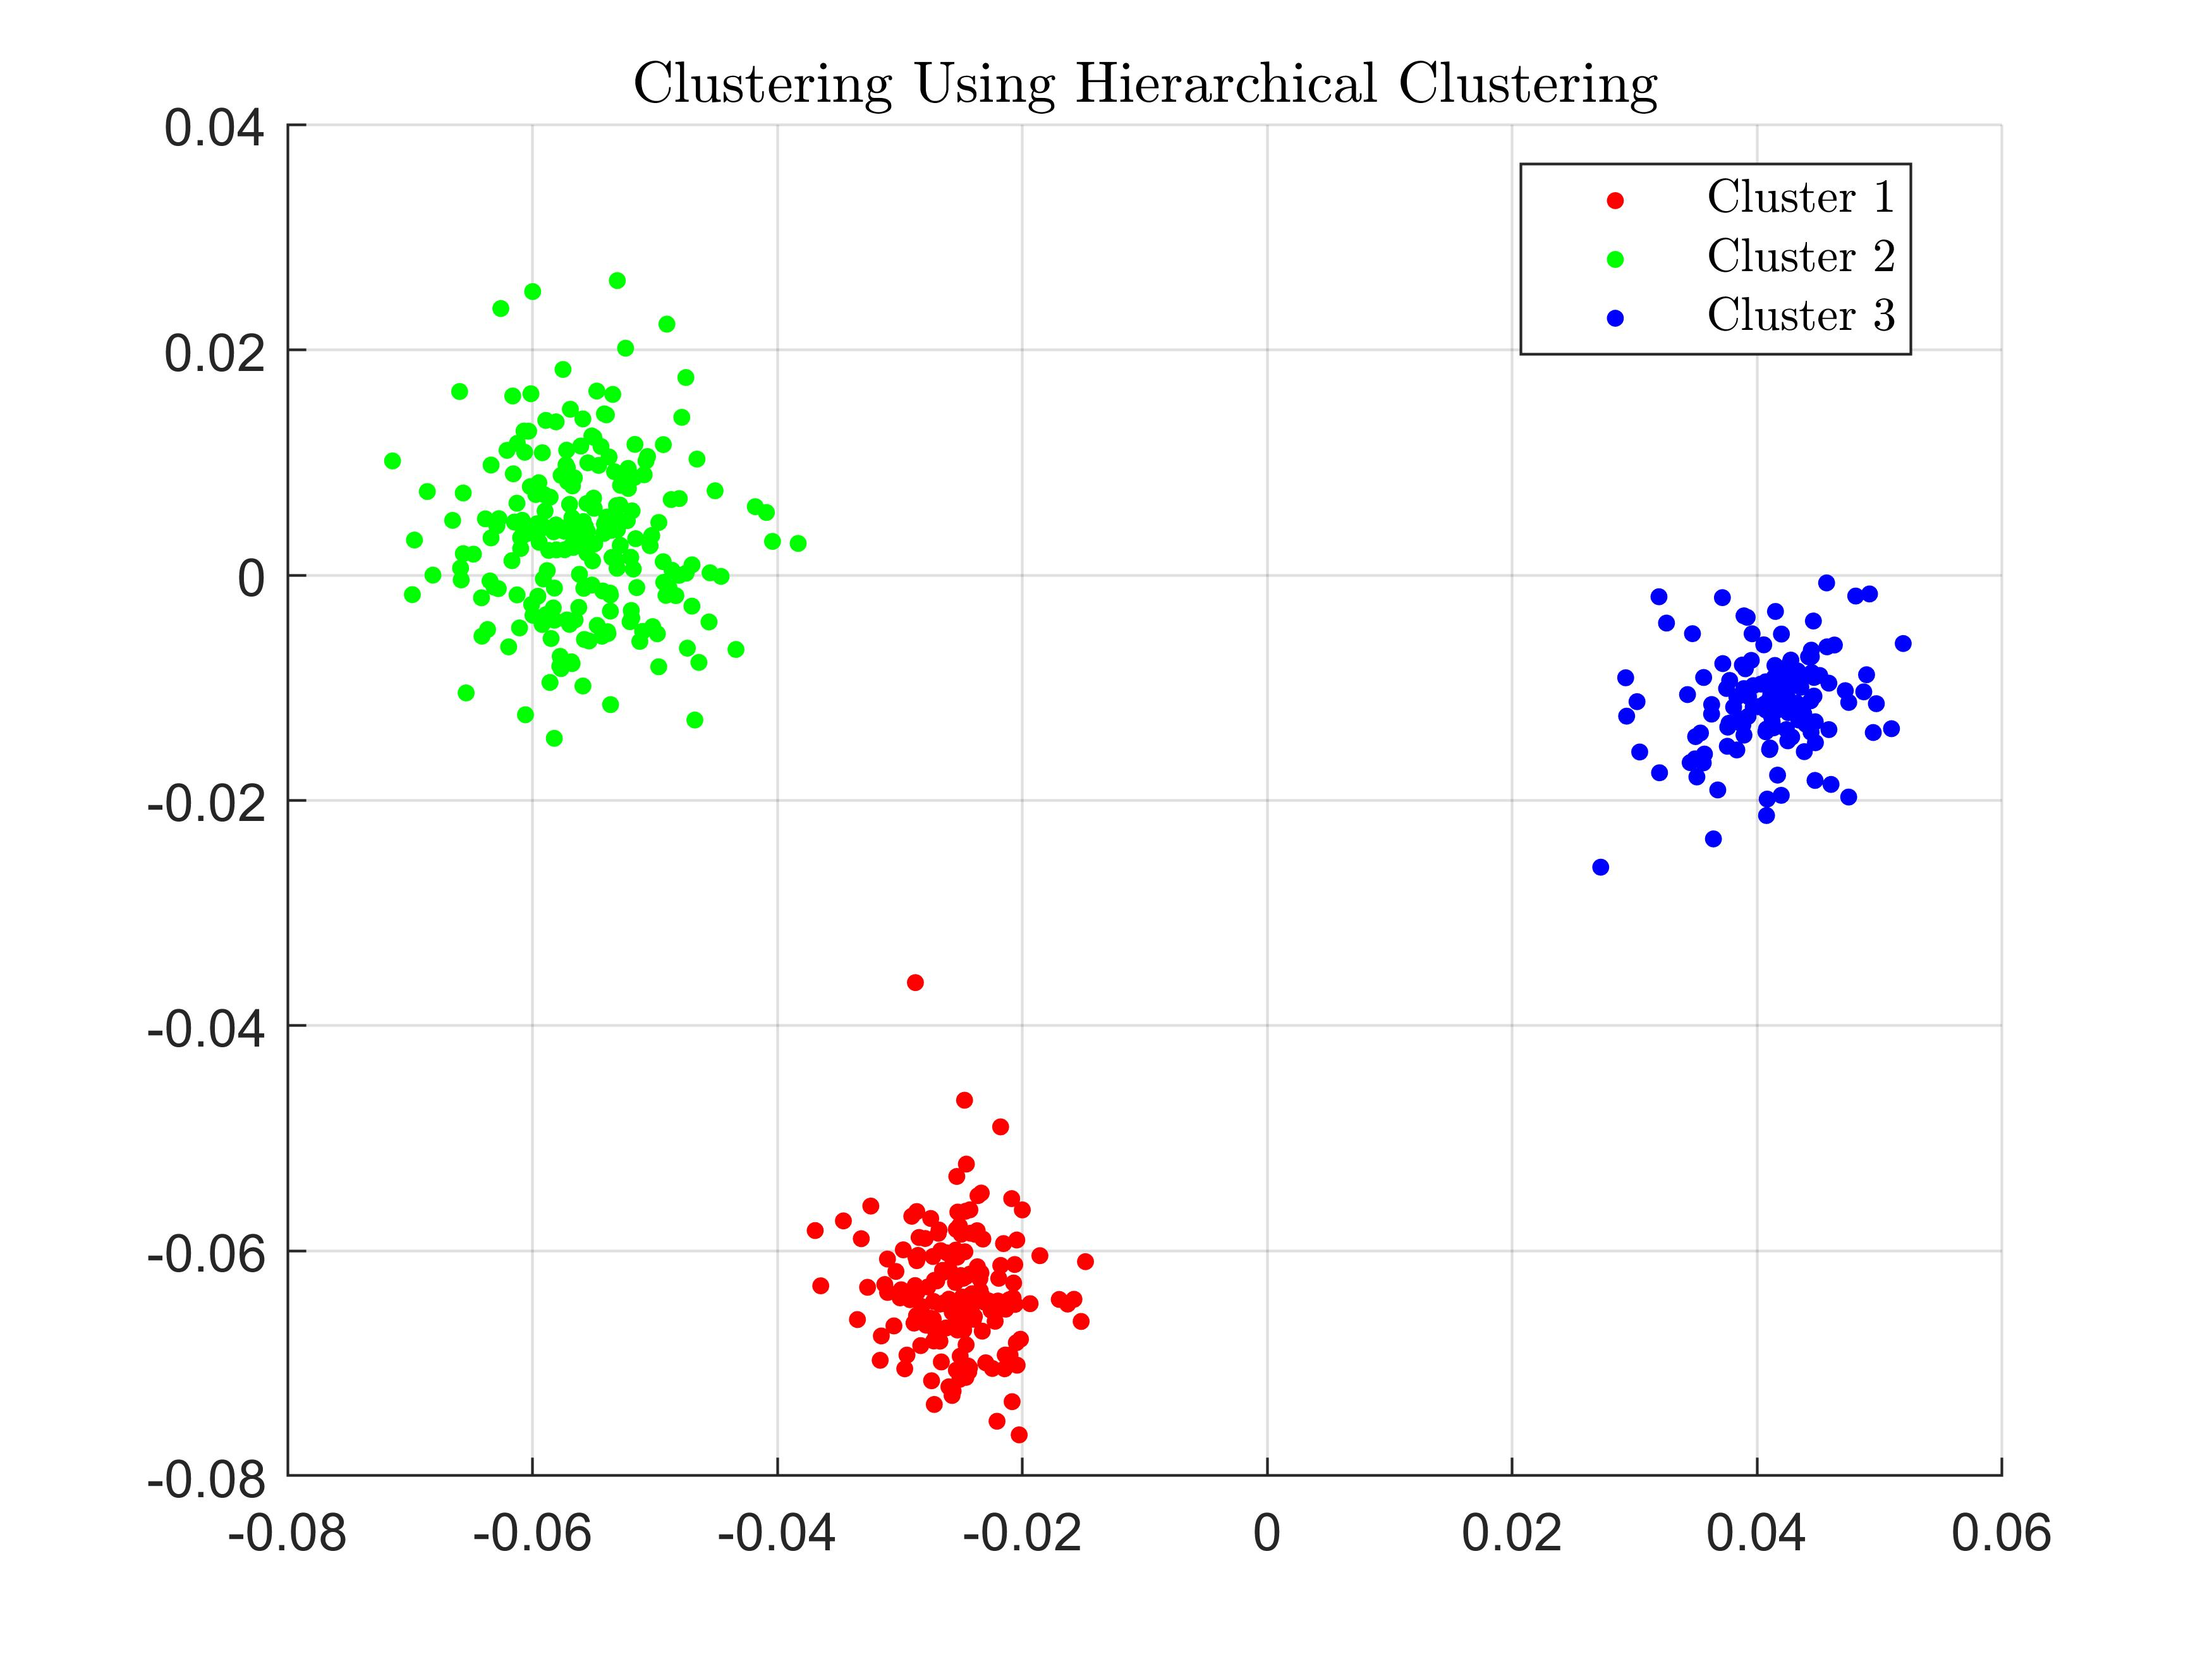
\includegraphics[width=0.9\textwidth]{HIERACHICAL2.jpg}
	\caption{Clustering Result Using Hierarchical Clustering after LDA}
	\label{fig:9}
\end{figure}

\hspace{0.7cm}
Since LDA has divided the class clearly, all the clustering methods perform well in this task, with different clusters exactly the different digits in MNIST dataset.

\subsection{PCA and LDA Using Larger MNIST Dataset}
\hspace{0.7cm}
Here I download the whole MNIST datasets with $60,000$ pictures form digit 0 to digit 9, and repeat the LDA and PCA to reduce the dimension to 2. The following results in Figure \ref{fig:10} and \ref{fig:11} are the dimensionality reduction plot using $2,000$ random pictures from the whole dataset, containing 10 different digits.

\hspace{0.7cm}
We can actually observe some interesting points in these 2 plots. For example, in the PCA 2-D plot, digit 0 distributes on the bottom, while digit 1 distributes on the top-right, we can guess maybe the direction on $y$ axis is finding curves and straight lines. However, in the center of PCA plot, there are many classes mixed together, making it difficult for us to do the classification, that is natural because PCA is an unsupervised algorithm. Comparatively, when we use LDA, which is a supervised algorithm, the data points of different classes are distributed in different regions in the final 2-D plot.

\begin{figure}[!htbp]
	\centering
	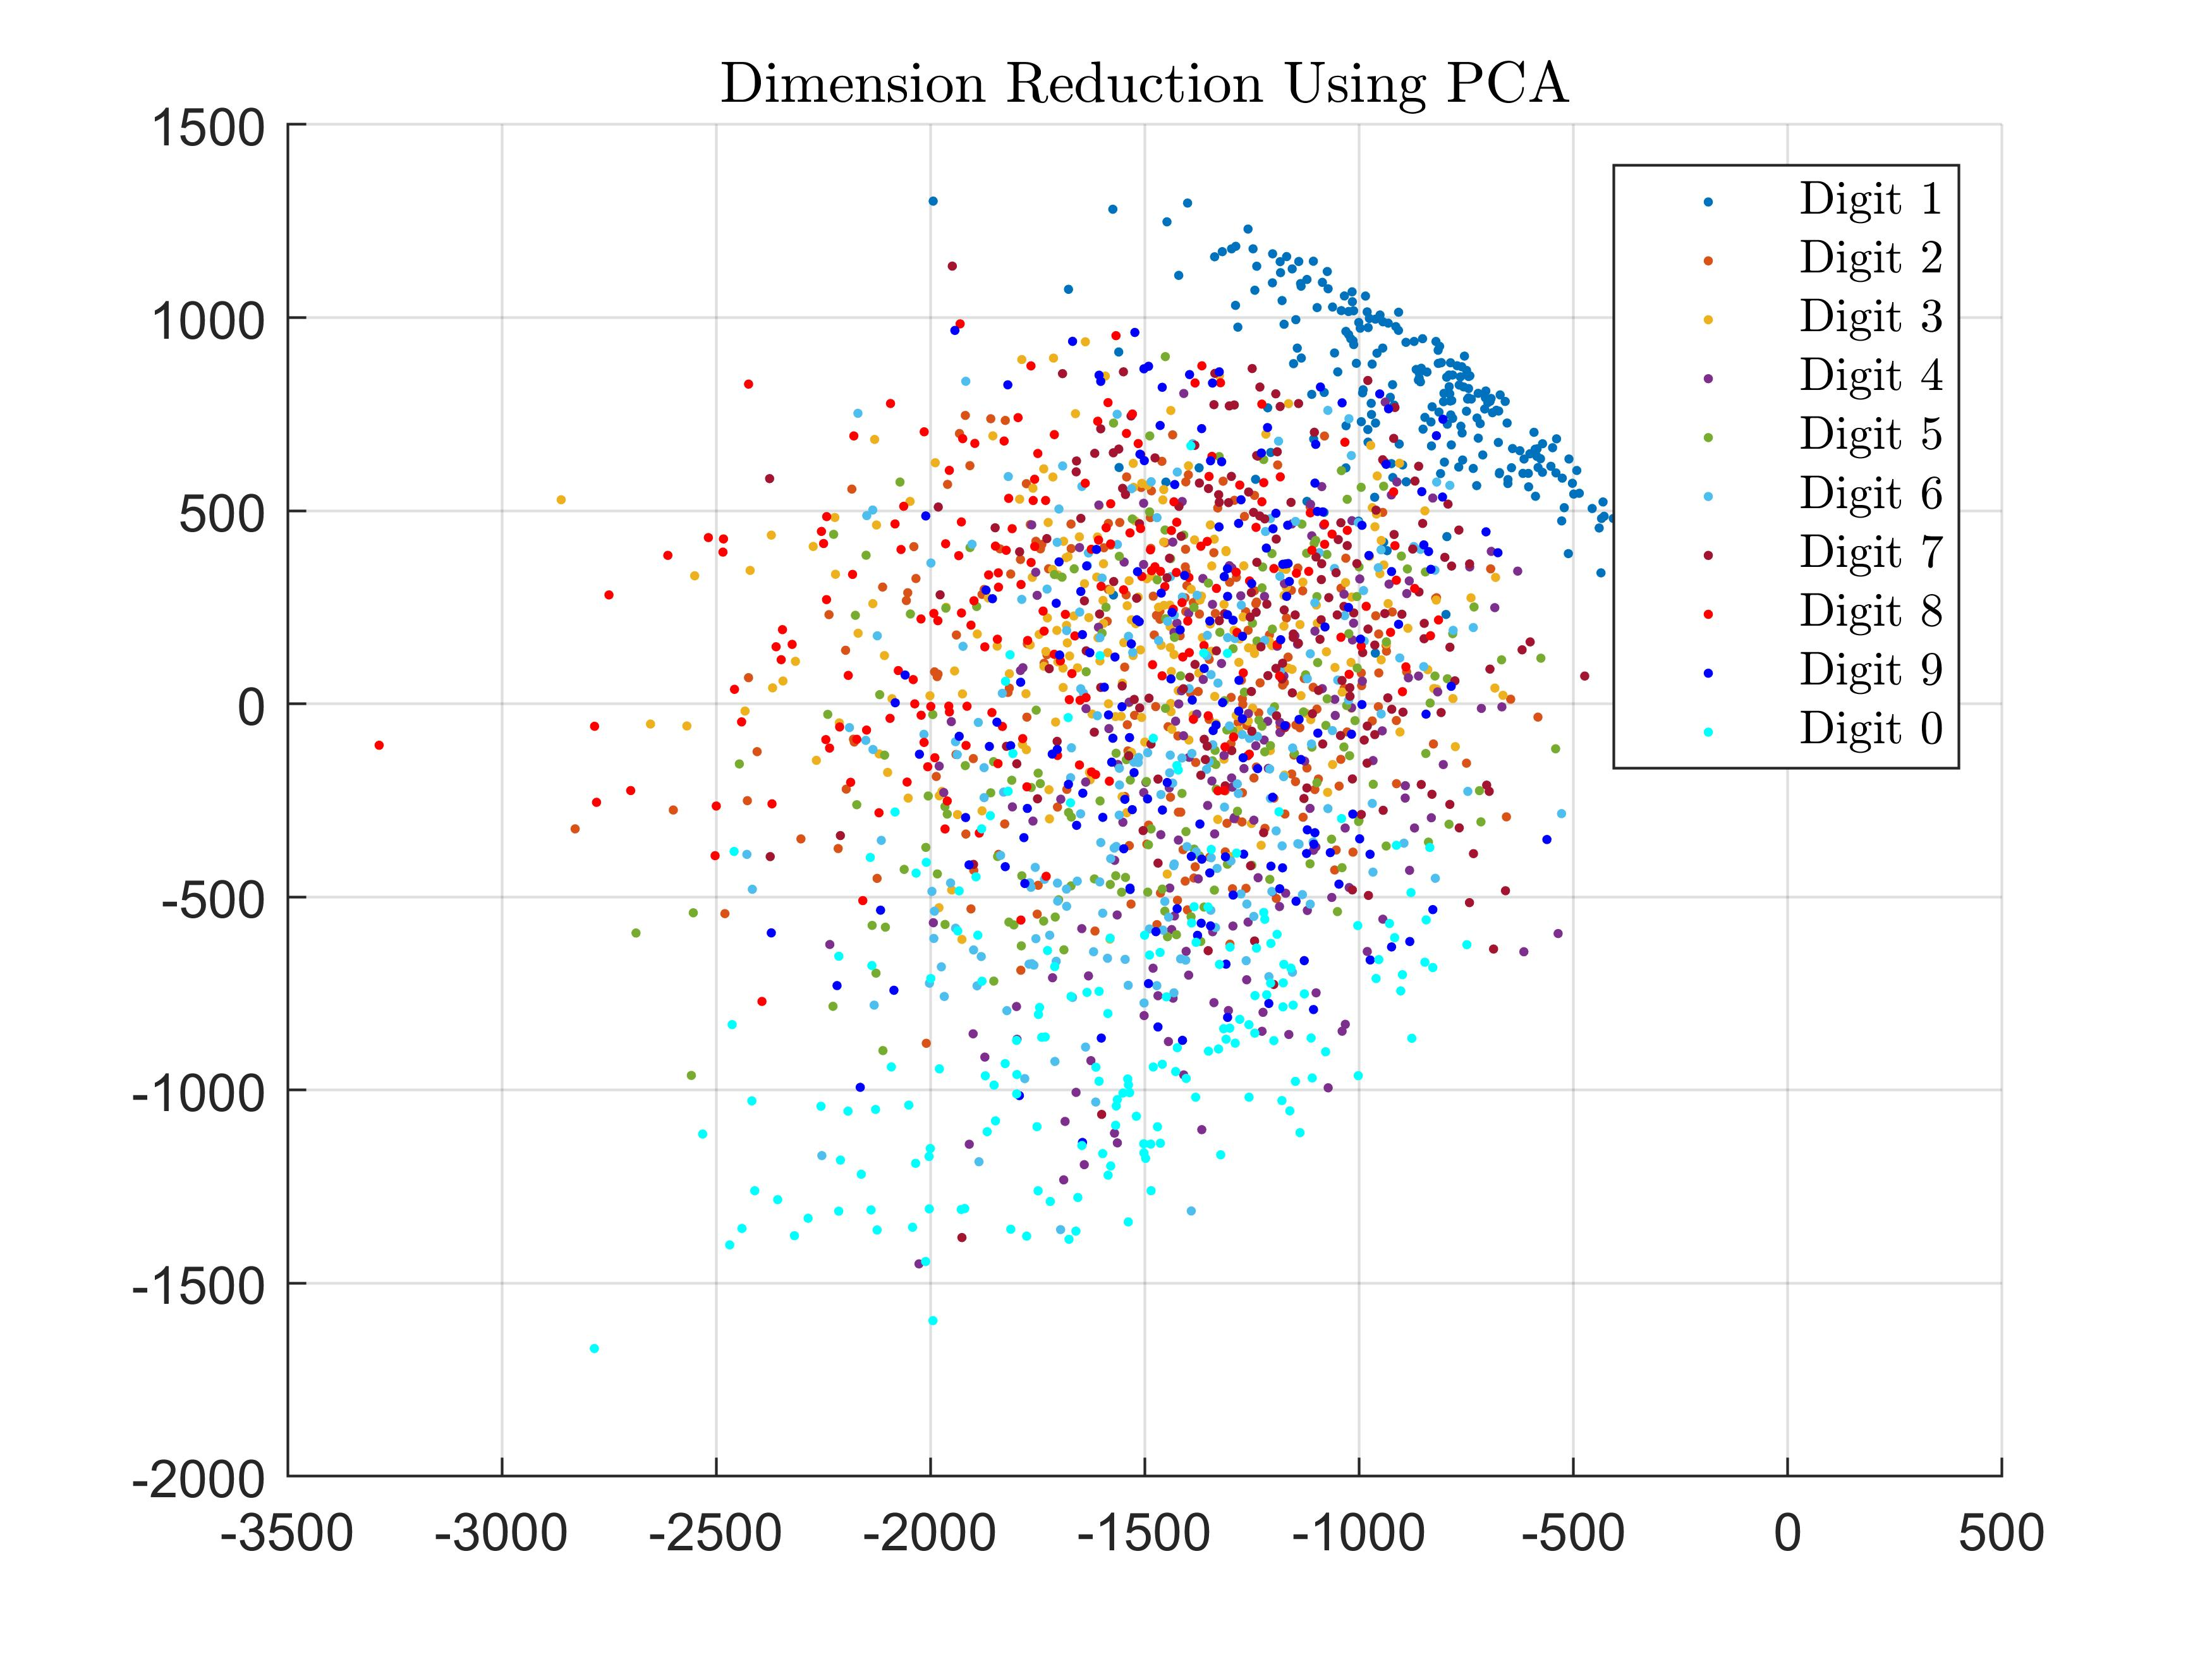
\includegraphics[width=0.9\textwidth]{PCAALL.jpg}
	\caption{Dimension Reduction Using PCA (2000 data points)}
	\label{fig:10}
\end{figure}

\begin{figure}[!htbp]
	\centering
	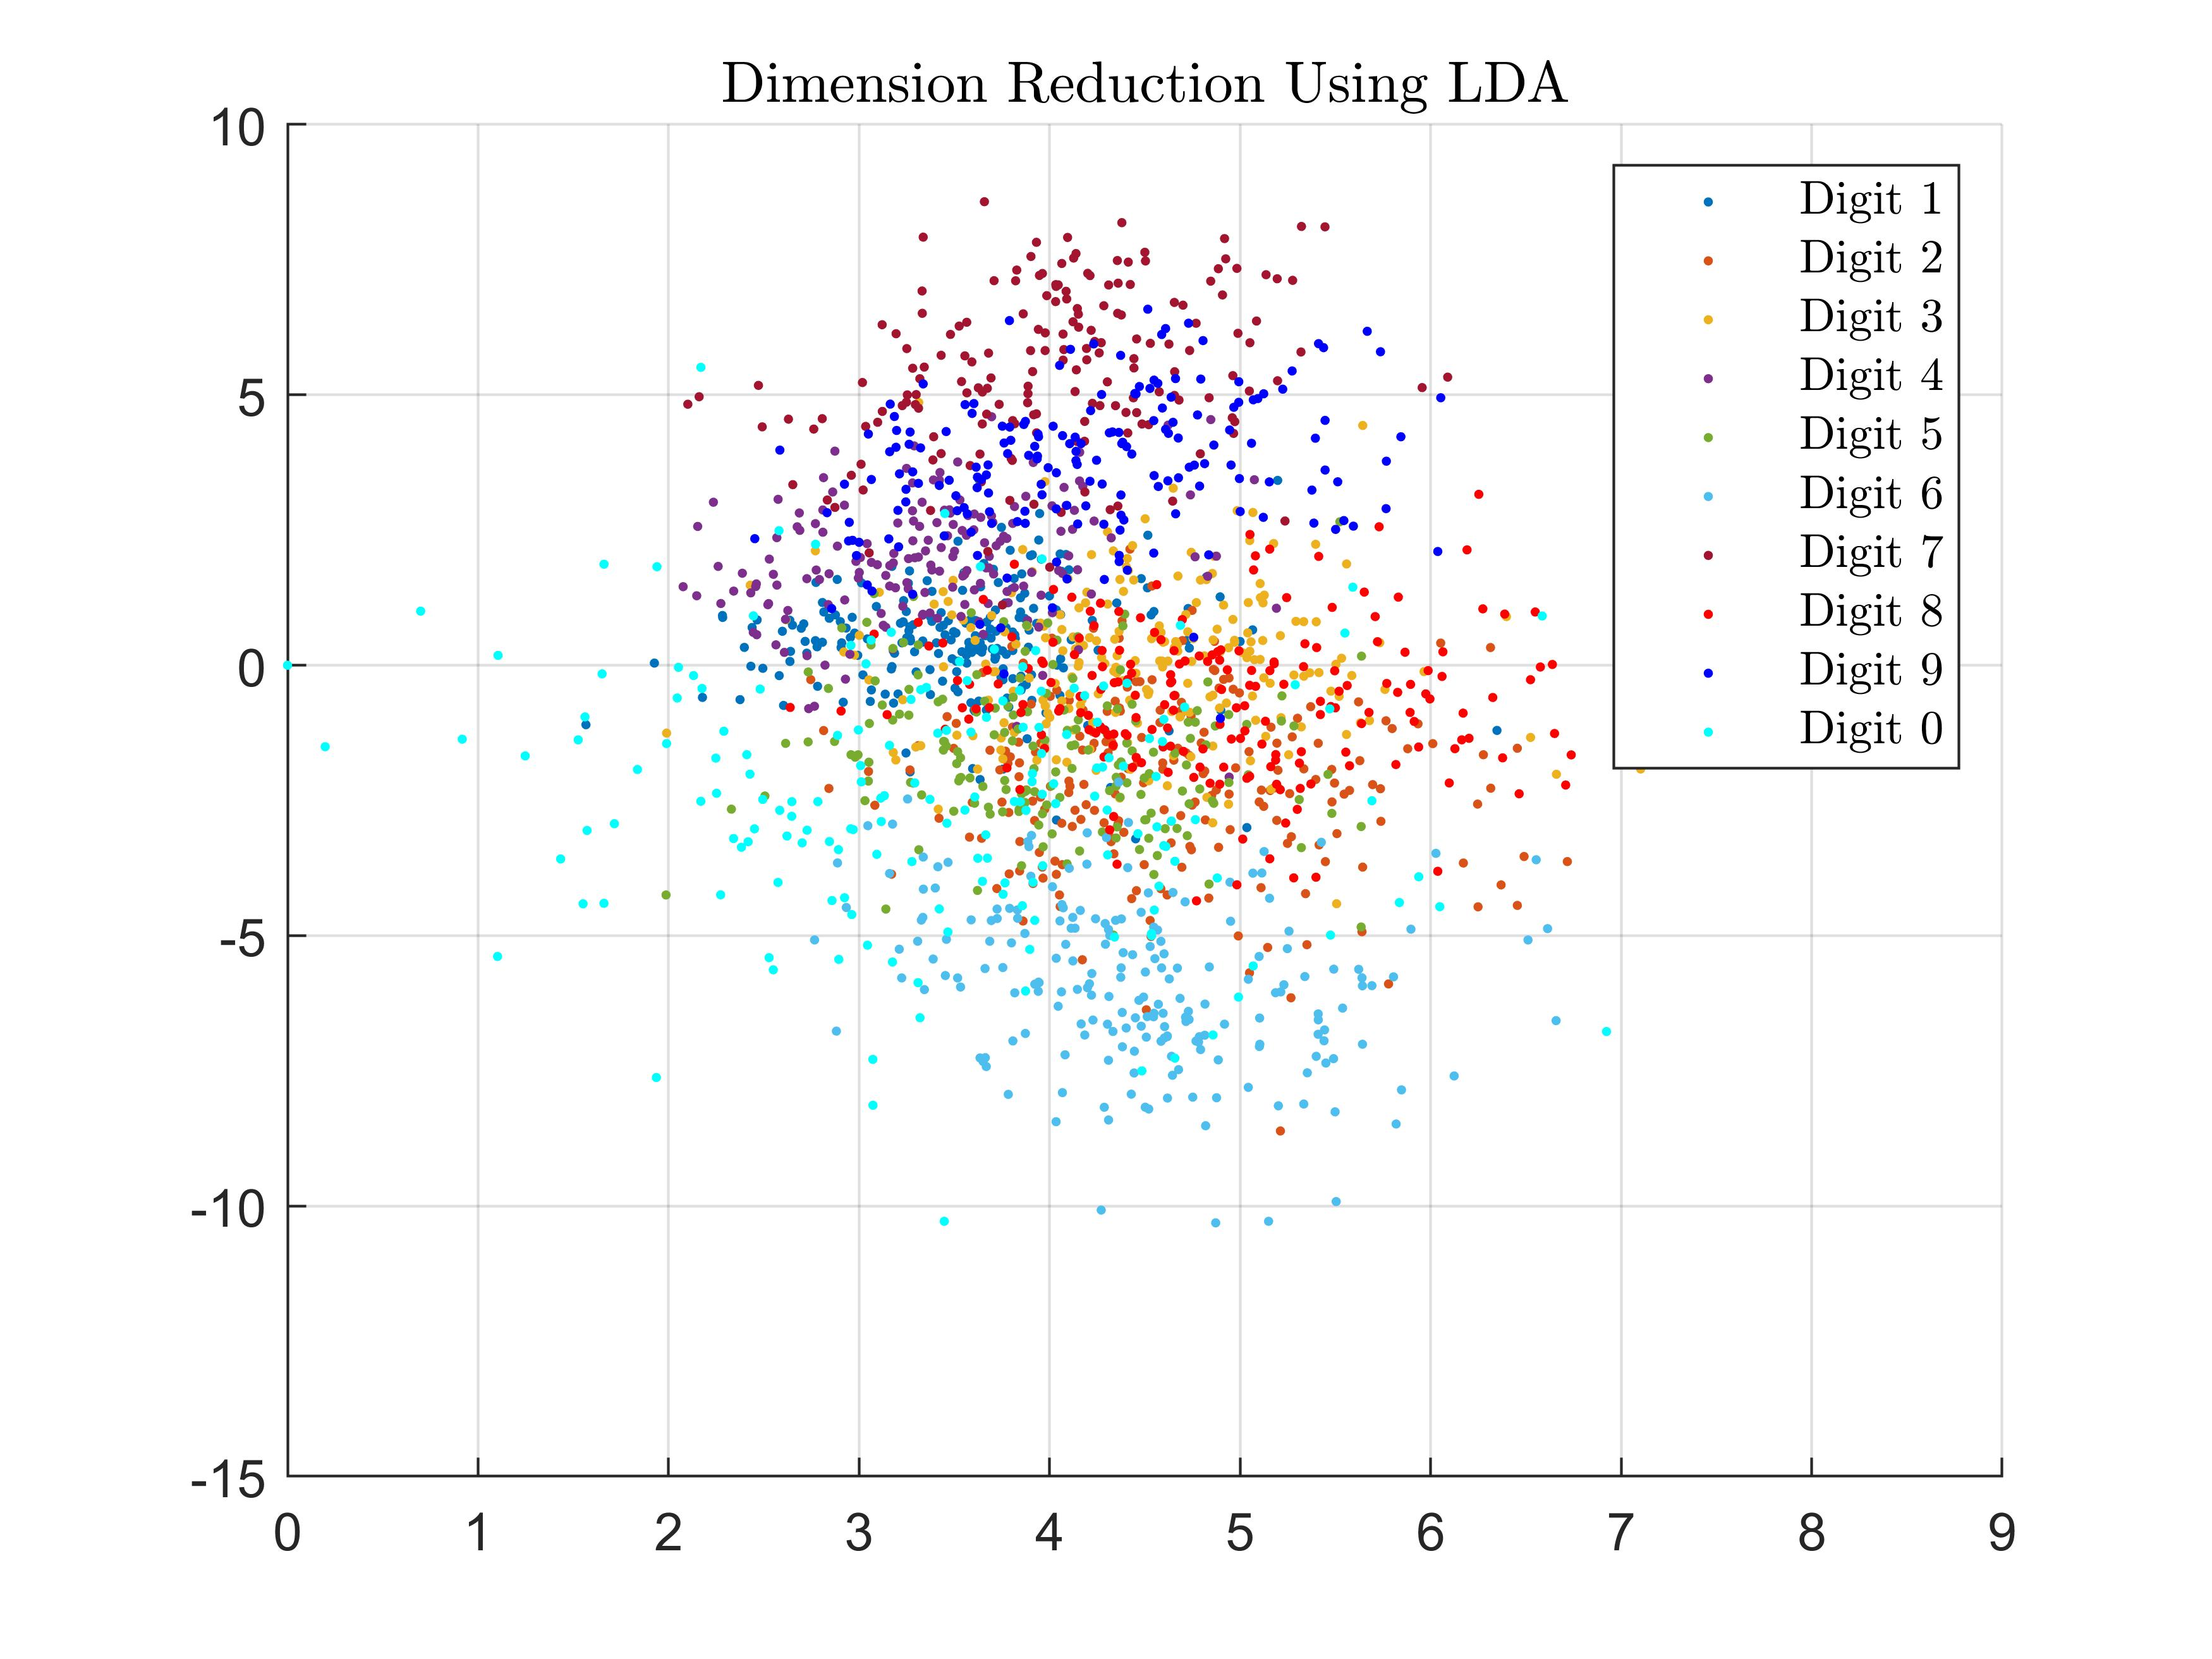
\includegraphics[width=0.9\textwidth]{LDAALL.jpg}
	\caption{Dimension Reduction Using LDA (2000 data points)}
	\label{fig:11}
\end{figure}

\section{Part II: Binary Classification}
\subsection{Preprocessing of Data, Cross-Validation Settings, Generating ROC Curves}
\hspace{0.7cm}
Firstly, we divide the dataset by digit 5 against others. Here I set digit 5 with label 1 and others with label 0.

\begin{footnotesize}
\begin{minted}[mathescape,breaklines,breakindent=0em,linenos,numbersep=5pt,gobble=0,framesep=2mm]{matlab}
% preparing the vectors for digit 5 against the rest
a = zeros(size(labels));
a(labels==5) = 1;
\end{minted}
\end{footnotesize}

\hspace{0.7cm}
I also use 5-fold cross-validation in this part to get a authentic accuracy to evaluate the model. The codes to implement the cross-validation process is given as below. To be noteworthy, we only divide the dataset once to guarantee the same division for different classifiers. That means, \texttt{cvpartition()} will only be executed once during this whole binary classification task.

\begin{footnotesize}
\begin{minted}[mathescape,breaklines,breakindent=0em,linenos,numbersep=5pt,gobble=0,framesep=2mm]{matlab}
% split the data into 5 fold.
cvo = cvpartition(a,'KFold',5);

predict_label_total = [];
test_label_vector_total = [];

% cross validation
accuracy_avg = 0;
for i = 1:5
trIdx = cvo.training(i); %% get the index of training samples
teIdx = cvo.test(i); %% get the index of the test samples
training_label_vector = a(trIdx); %% creating the training label
%ground truth
training_instance_matrix = images(trIdx,:); %% creating the training
%data matrix
test_label_vector = a(teIdx); %% creating the testing label
%ground truth
test_instance_matrix = images(teIdx,:); %% creating the test data

train...
predict...

predict_label_total = [predict_label_total; predict_label];
test_label_vector_total = [test_label_vector_total; test_label_vector];
end
% cross validation accuracy
accuracy_avg = accuracy_avg / 5;
\end{minted}
\end{footnotesize}

\hspace{0.7cm}
I also try to plot the ROC curves and calculate the area under the curve (AUC) by myself using a self-written MATLAB function.

\begin{footnotesize}
\begin{minted}[mathescape,breaklines,breakindent=0em,linenos,numbersep=5pt,gobble=0,framesep=2mm]{matlab}
function  auc = plot_roc(predict, ground_truth)
% plot the ROC curve

x = 1.0;
y = 1.0;

%calculate numbers of positive and negative samples
pos_num = sum(ground_truth==1);
neg_num = sum(ground_truth==0);

%calculate step size for plot
x_step = 1.0/neg_num;
y_step = 1.0/pos_num;

%sort the output value
[~,index] = sort(predict);
ground_truth = ground_truth(index);

%plot the ROC curve
for i=1:length(ground_truth)
    if ground_truth(i) == 1
        y = y - y_step;
    else
        x = x - x_step;
    end
    X(i)=x;
    Y(i)=y;
end

hold on;
grid on;
set(gcf,'Position',[50/0.277 50/0.277 100/0.277 100/0.277]);
plot(X,Y,'-b','LineWidth',2,'MarkerSize',3);
plot(X,X,'--k','LineWidth',0.5)
xlim([0 1]); ylim([0 1]);

xlabel('False Positive Rate', 'Interpreter', 'latex');
ylabel('True Positive Rate', 'Interpreter', 'latex');
title('ROC Curve', 'Interpreter', 'latex');
%calculate the area under ROC curve, i.e. auc
auc = -trapz(X,Y);
end
\end{minted}
\end{footnotesize}

\subsection{SVM with RBF Kernal}
\hspace{0.7cm}
I trained a SVM with RBF kernal ($\gamma =0.07$) and evaluated the performance by using the \texttt{svmtrain()} and \texttt{svmpredict()}.

\begin{footnotesize}
\begin{minted}[mathescape,breaklines,breakindent=0em,linenos,numbersep=5pt,gobble=0,framesep=2mm]{matlab}
model = svmtrain(training_label_vector, training_instance_matrix, '-t 2 -g 0.07');
[predict_label, accuracy, dec_values] = svmpredict(test_label_vector, test_instance_matrix, model);
\end{minted}
\end{footnotesize}

\hspace{0.7cm}
The average accuracy after 5-fold cross-validation is \textbf{97.83\%}. Area under the ROC curve AUC is \textbf{0.9710}. The ROC curve is shwn in Figure \ref{fig:roc1}.

\begin{figure}[!htbp]
	\centering
	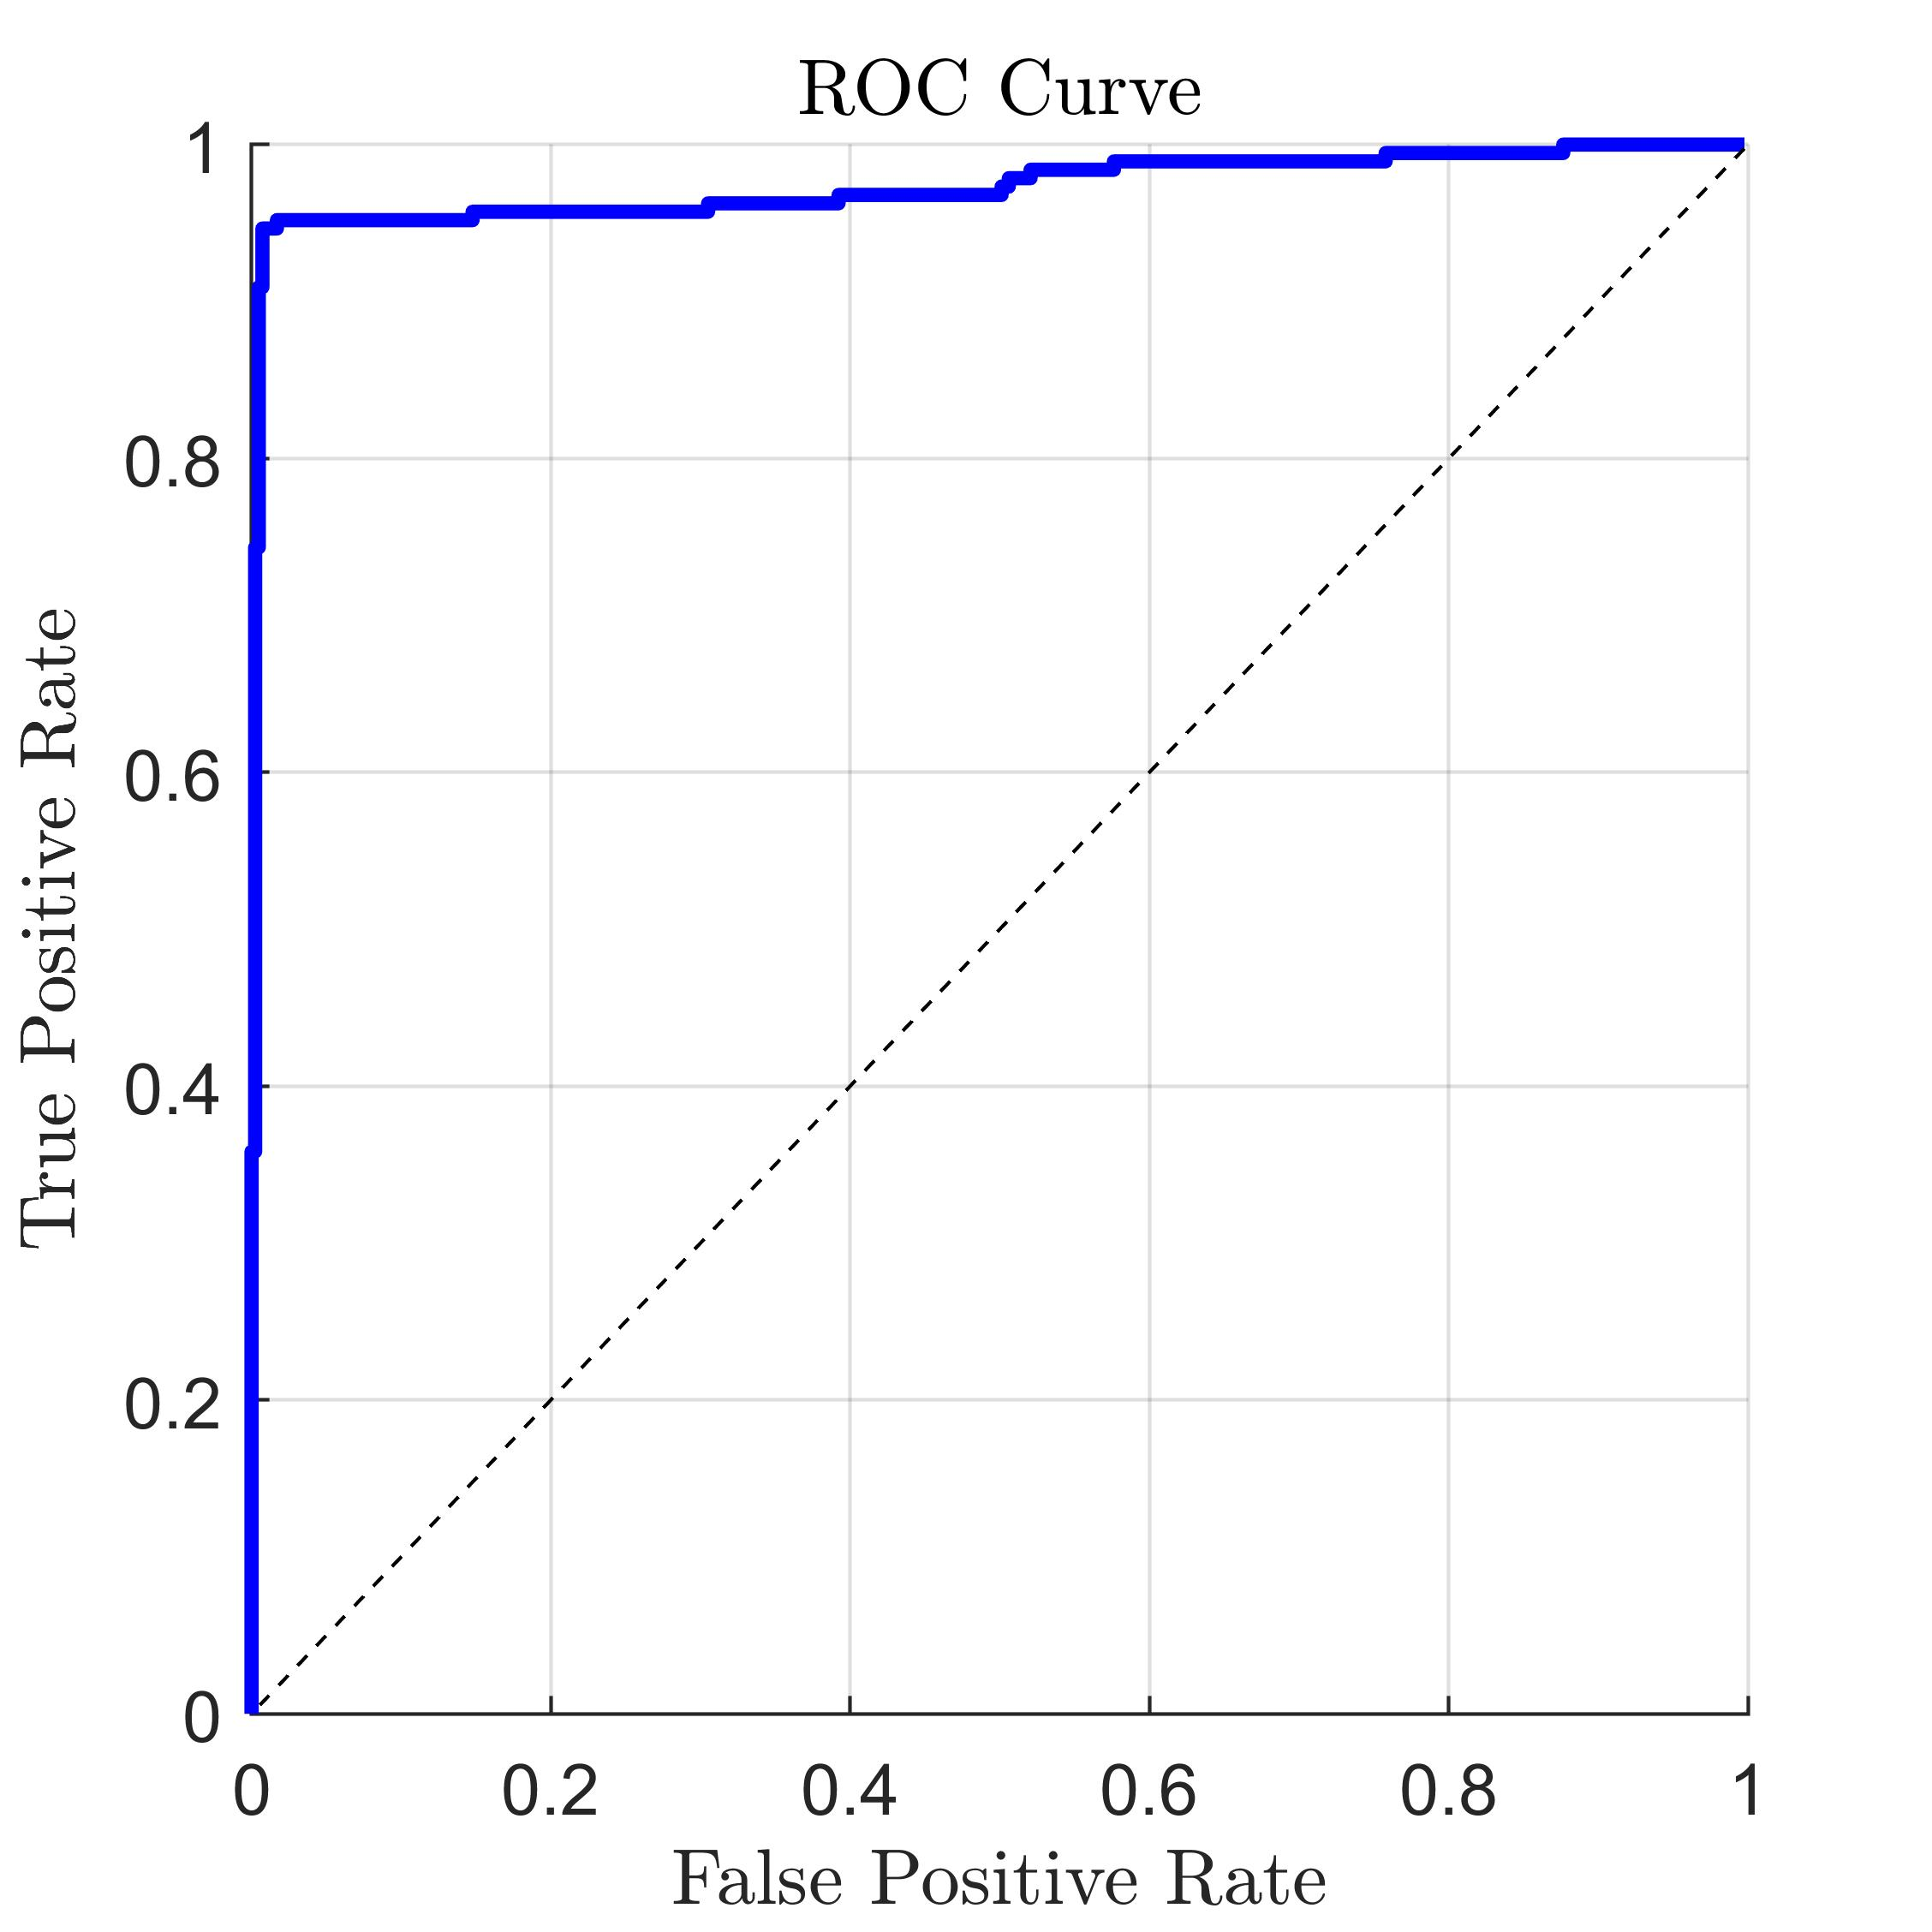
\includegraphics[width=0.5\textwidth]{RBFROC.jpg}
	\caption{ROC Curve of SVM with RBF Kernal}
	\label{fig:roc1}
\end{figure}

\subsection{SVM with Linear Kernal}
\hspace{0.7cm}
In this part, I trained a SVM with linear kernal and evaluated the performance by using the \texttt{svmtrain()} and \texttt{svmpredict()}. The goal of SVM is to find a line that can have the maximum spread with the data points. RBF kernal is common in defining SVM, it provides nonlinerity for the classification regions.

\begin{figure}[!htbp]
	\centering
	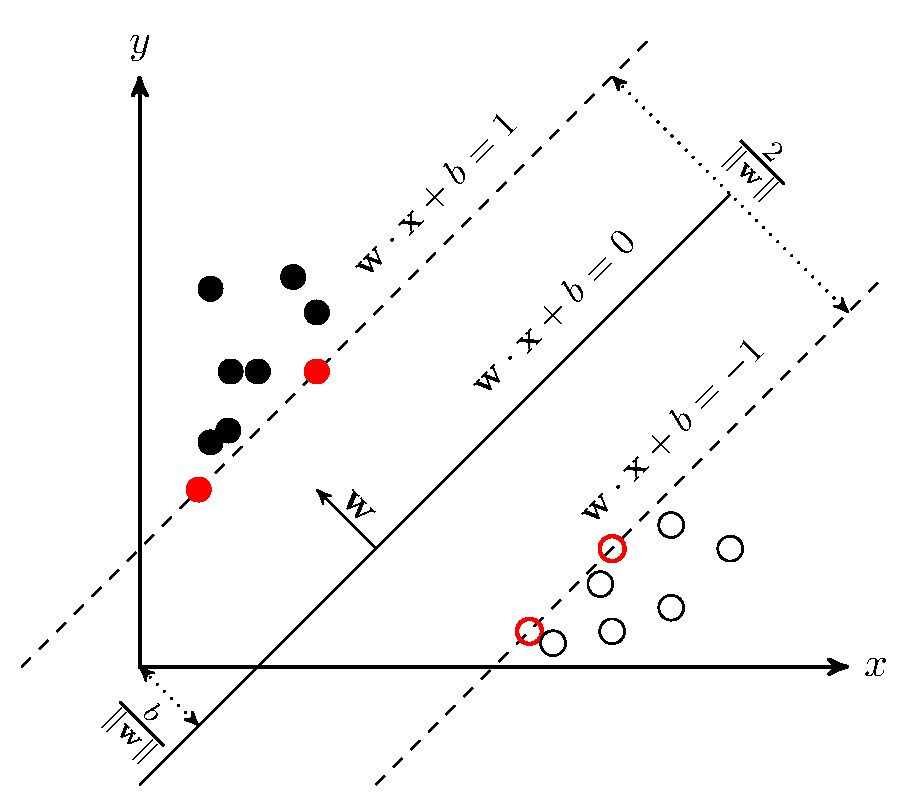
\includegraphics[width=0.5\textwidth]{SVM.png}
	\caption{Schematic Plot of SVM}
\end{figure}

\begin{footnotesize}
\begin{minted}[mathescape,breaklines,breakindent=0em,linenos,numbersep=5pt,gobble=0,framesep=2mm]{matlab}
model = svmtrain(training_label_vector, training_instance_matrix, '-t 0');
[predict_label, accuracy, dec_values] = svmpredict(test_label_vector, test_instance_matrix, model);
\end{minted}
\end{footnotesize}

\hspace{0.7cm}
The average accuracy after 5-fold cross-validation is \textbf{95.00\%}. Area under the ROC curve AUC is \textbf{0.9420}. The ROC curve is shwn in Figure \ref{fig:roc2}.

\begin{figure}[!htbp]
	\centering
	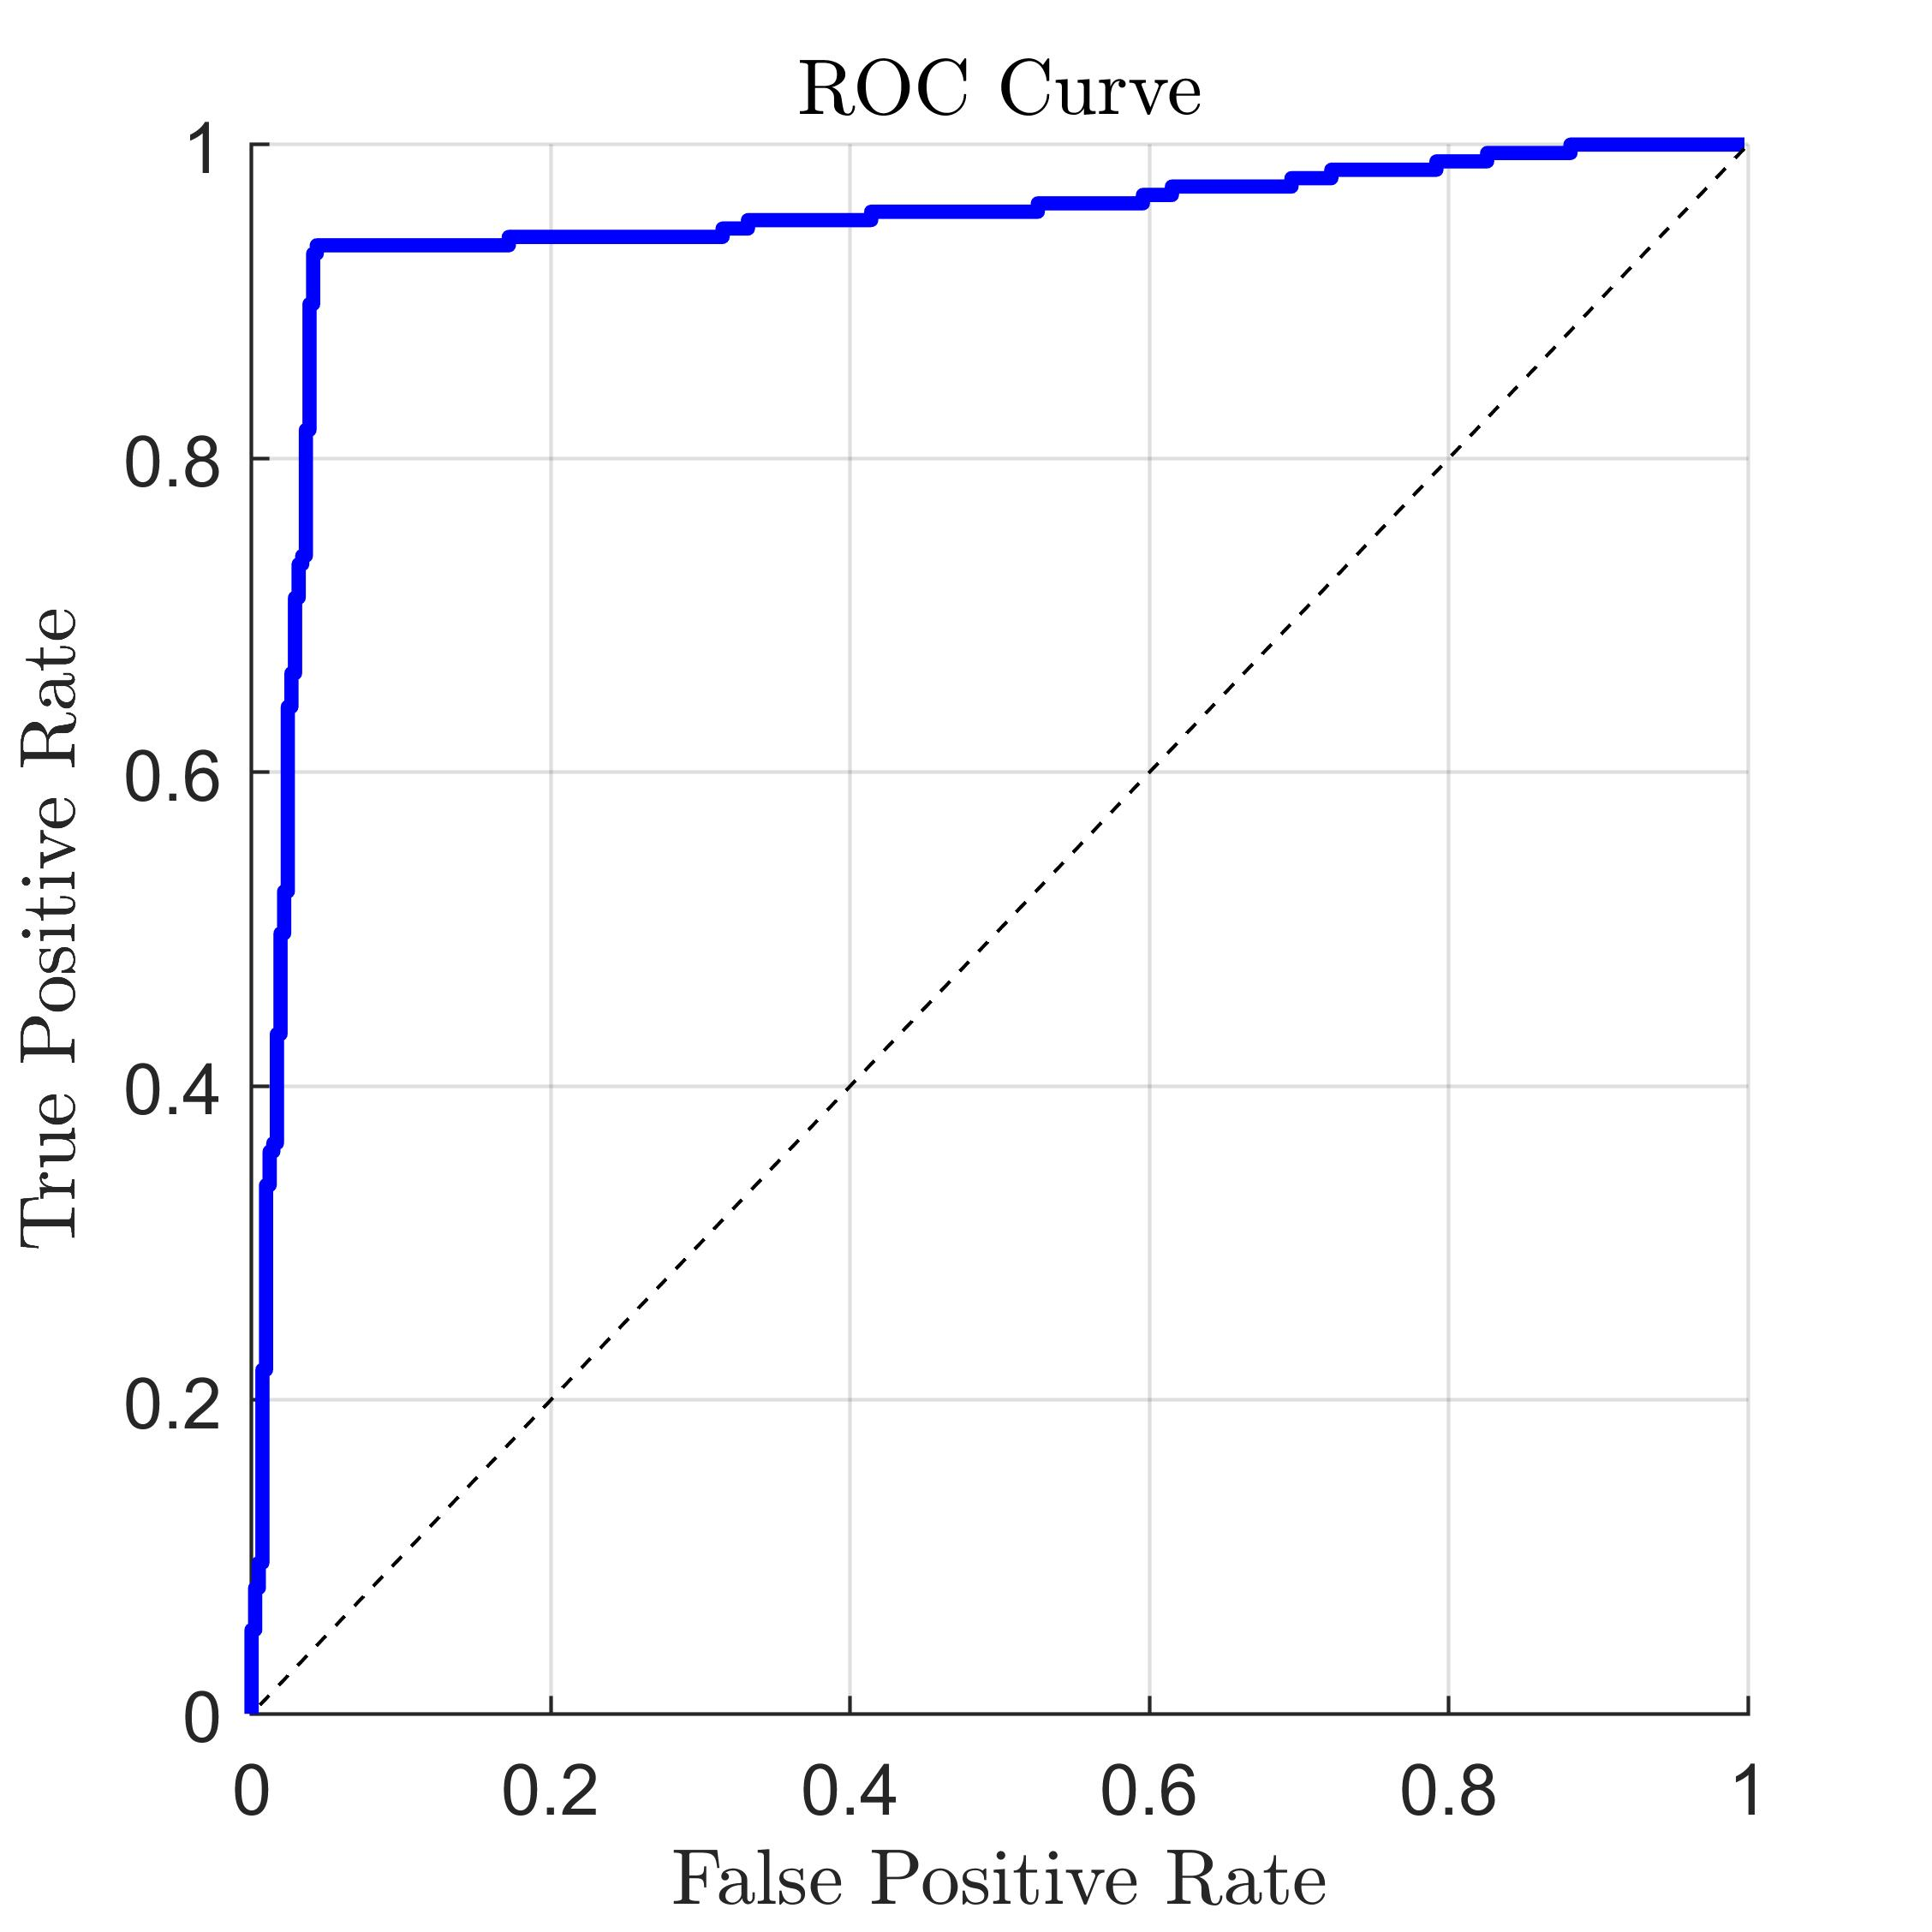
\includegraphics[width=0.5\textwidth]{LROC.jpg}
	\caption{ROC Curve of SVM with Linear Kernal}
	\label{fig:roc2}
\end{figure}

\subsection{Neural Network}
\hspace{0.7cm}
In this part, I trained a neural network with 1 hidden layer with sigmoid activation function and SGD, evaluated the performance by using the \texttt{feedforwardnet()}. The related codes are attached.

\begin{figure}[!htbp]
	\centering
	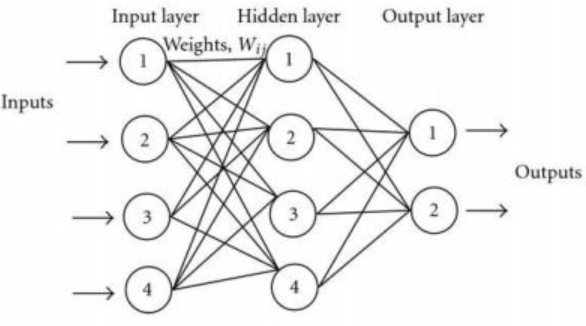
\includegraphics[width=0.65\textwidth]{NN.png}
	\caption{Schematic Plot of Neural Network}
	\label{fig:roc3}
\end{figure}

\begin{footnotesize}
\begin{minted}[mathescape,breaklines,breakindent=0em,linenos,numbersep=5pt,gobble=0,framesep=2mm]{matlab}
% Configure the net
net.divideParam.trainRatio = 1; % training set [%]
net.divideParam.valRatio = 0; % validation set [%]
net.divideParam.testRatio = 0; % test set [%]
net.inputs{1}.processFcns = {}; % modify the process function for inputs
net.outputs{2}.processFcns = {}; % modify the process function for outputs
net.layers{1}.transferFcn = 'logsig'; % the transfer function for the first layer
net.layers{2}.transferFcn = 'logsig'; % the transfer function for the second layer
net.trainParam.lr = 0.3; % learning rate. You may need to adjust it in the experiment.

% train the network
net = train(net, training_instance_matrix', training_label_vector');
\end{minted}
\end{footnotesize}

\hspace{0.7cm}
The average accuracy after 5-fold cross-validation is \textbf{95.27\%}. Area under the ROC curve AUC is \textbf{0.9737}. The ROC curve is shwn in Figure \ref{fig:roc4}.

\begin{figure}[!htbp]
	\centering
	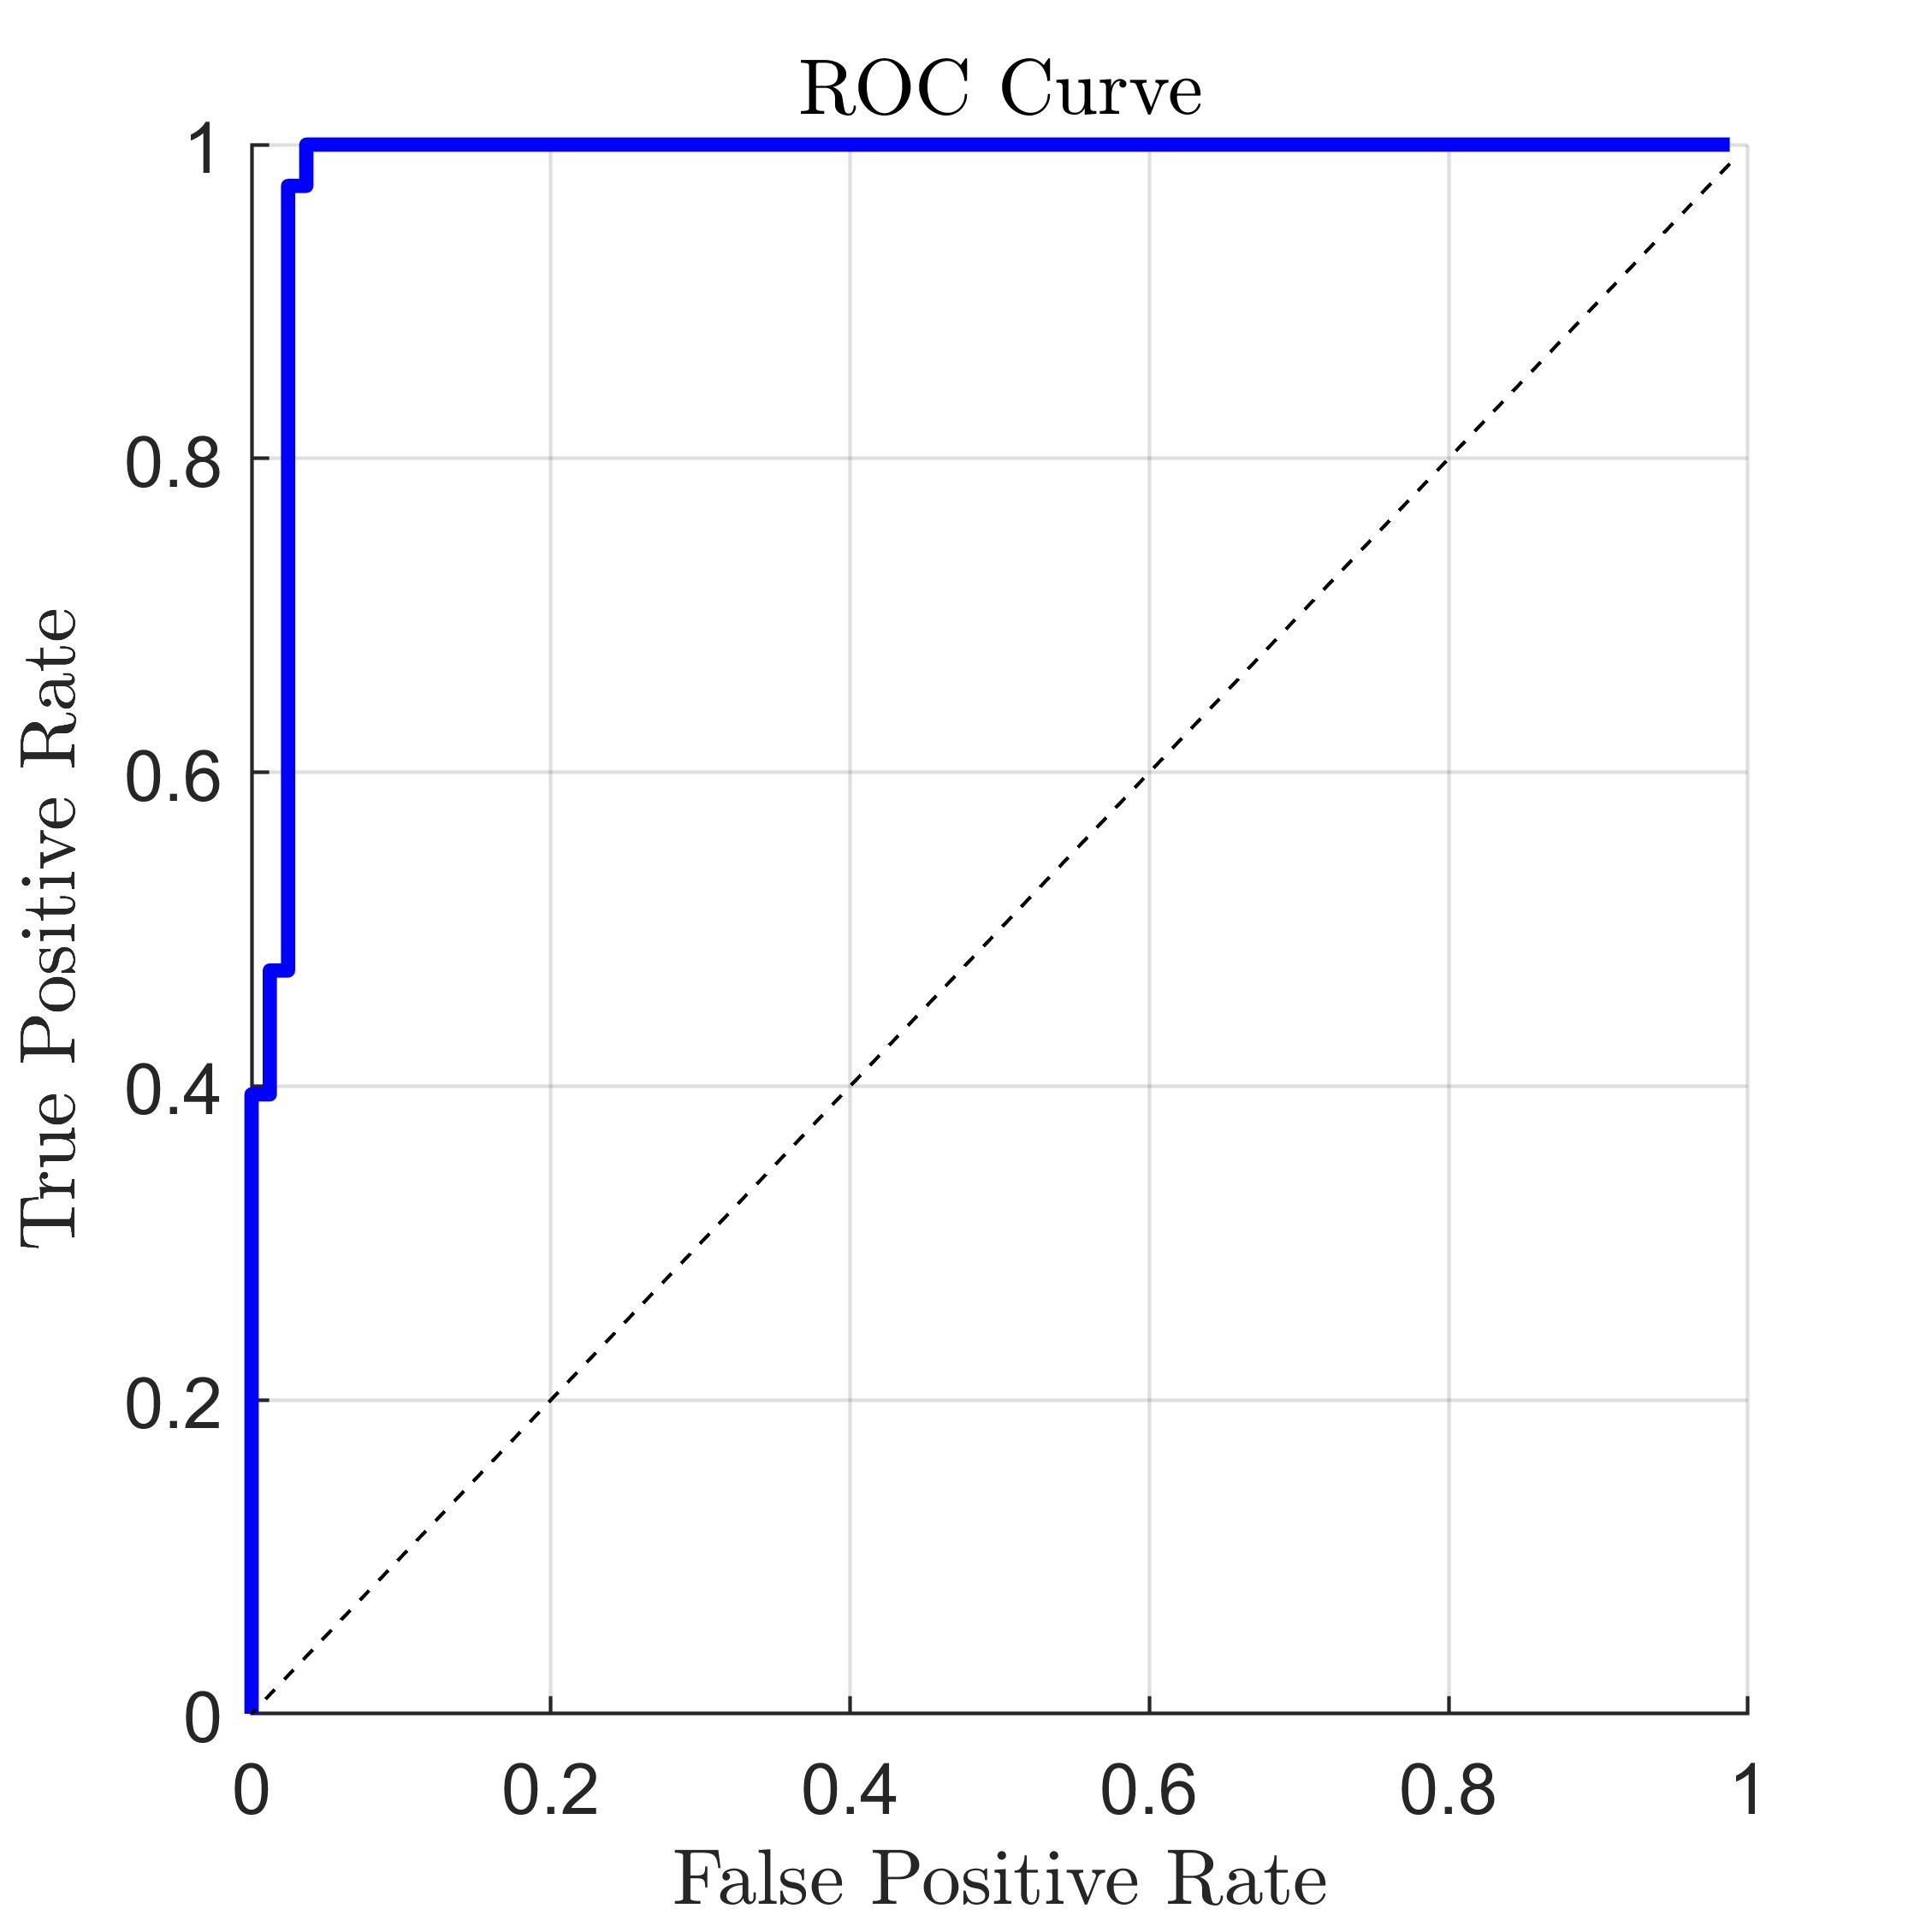
\includegraphics[width=0.5\textwidth]{NNROC.jpg}
	\caption{ROC Curve of Neural Network}
	\label{fig:roc4}
\end{figure}

\subsection{Summary}
\hspace{0.7cm}
To summarize, SVM with RBF kernal performs the best in such division of dataset, while the neural network has the greatest AUC, which means it can do well in almost all the thresholds. SVM with linear kernal performs badly in this experiment. However, all these 3 models have a AUC much greater than 0.5, which is the AUC of random guess.

\subsection{Fine-Tune the Parameters}
\hspace{0.7cm}
Here we choose to fine-tune the hyperparameter $\gamma$ in SVM with RBF kernal. We list the possible candidates for $\gamma$.

\begin{footnotesize}
\begin{minted}[mathescape,breaklines,breakindent=0em,linenos,numbersep=5pt,gobble=0,framesep=2mm]{matlab}
gamma_choices = [0.001, 0.007, 0.02, 0.035, 0.05, 0.07, 0.1];
\end{minted}
\end{footnotesize}

\hspace{0.7cm}
For each candidate, we plot the ROC curves, get the AUC and calculate the average cross-validation accuracy in 3 different 5-fold cross validation settings. The experiment result is given in Figure \ref{fig:ft} and \ref{fig:ft2}.


\begin{figure}[!htbp]
	\centering
	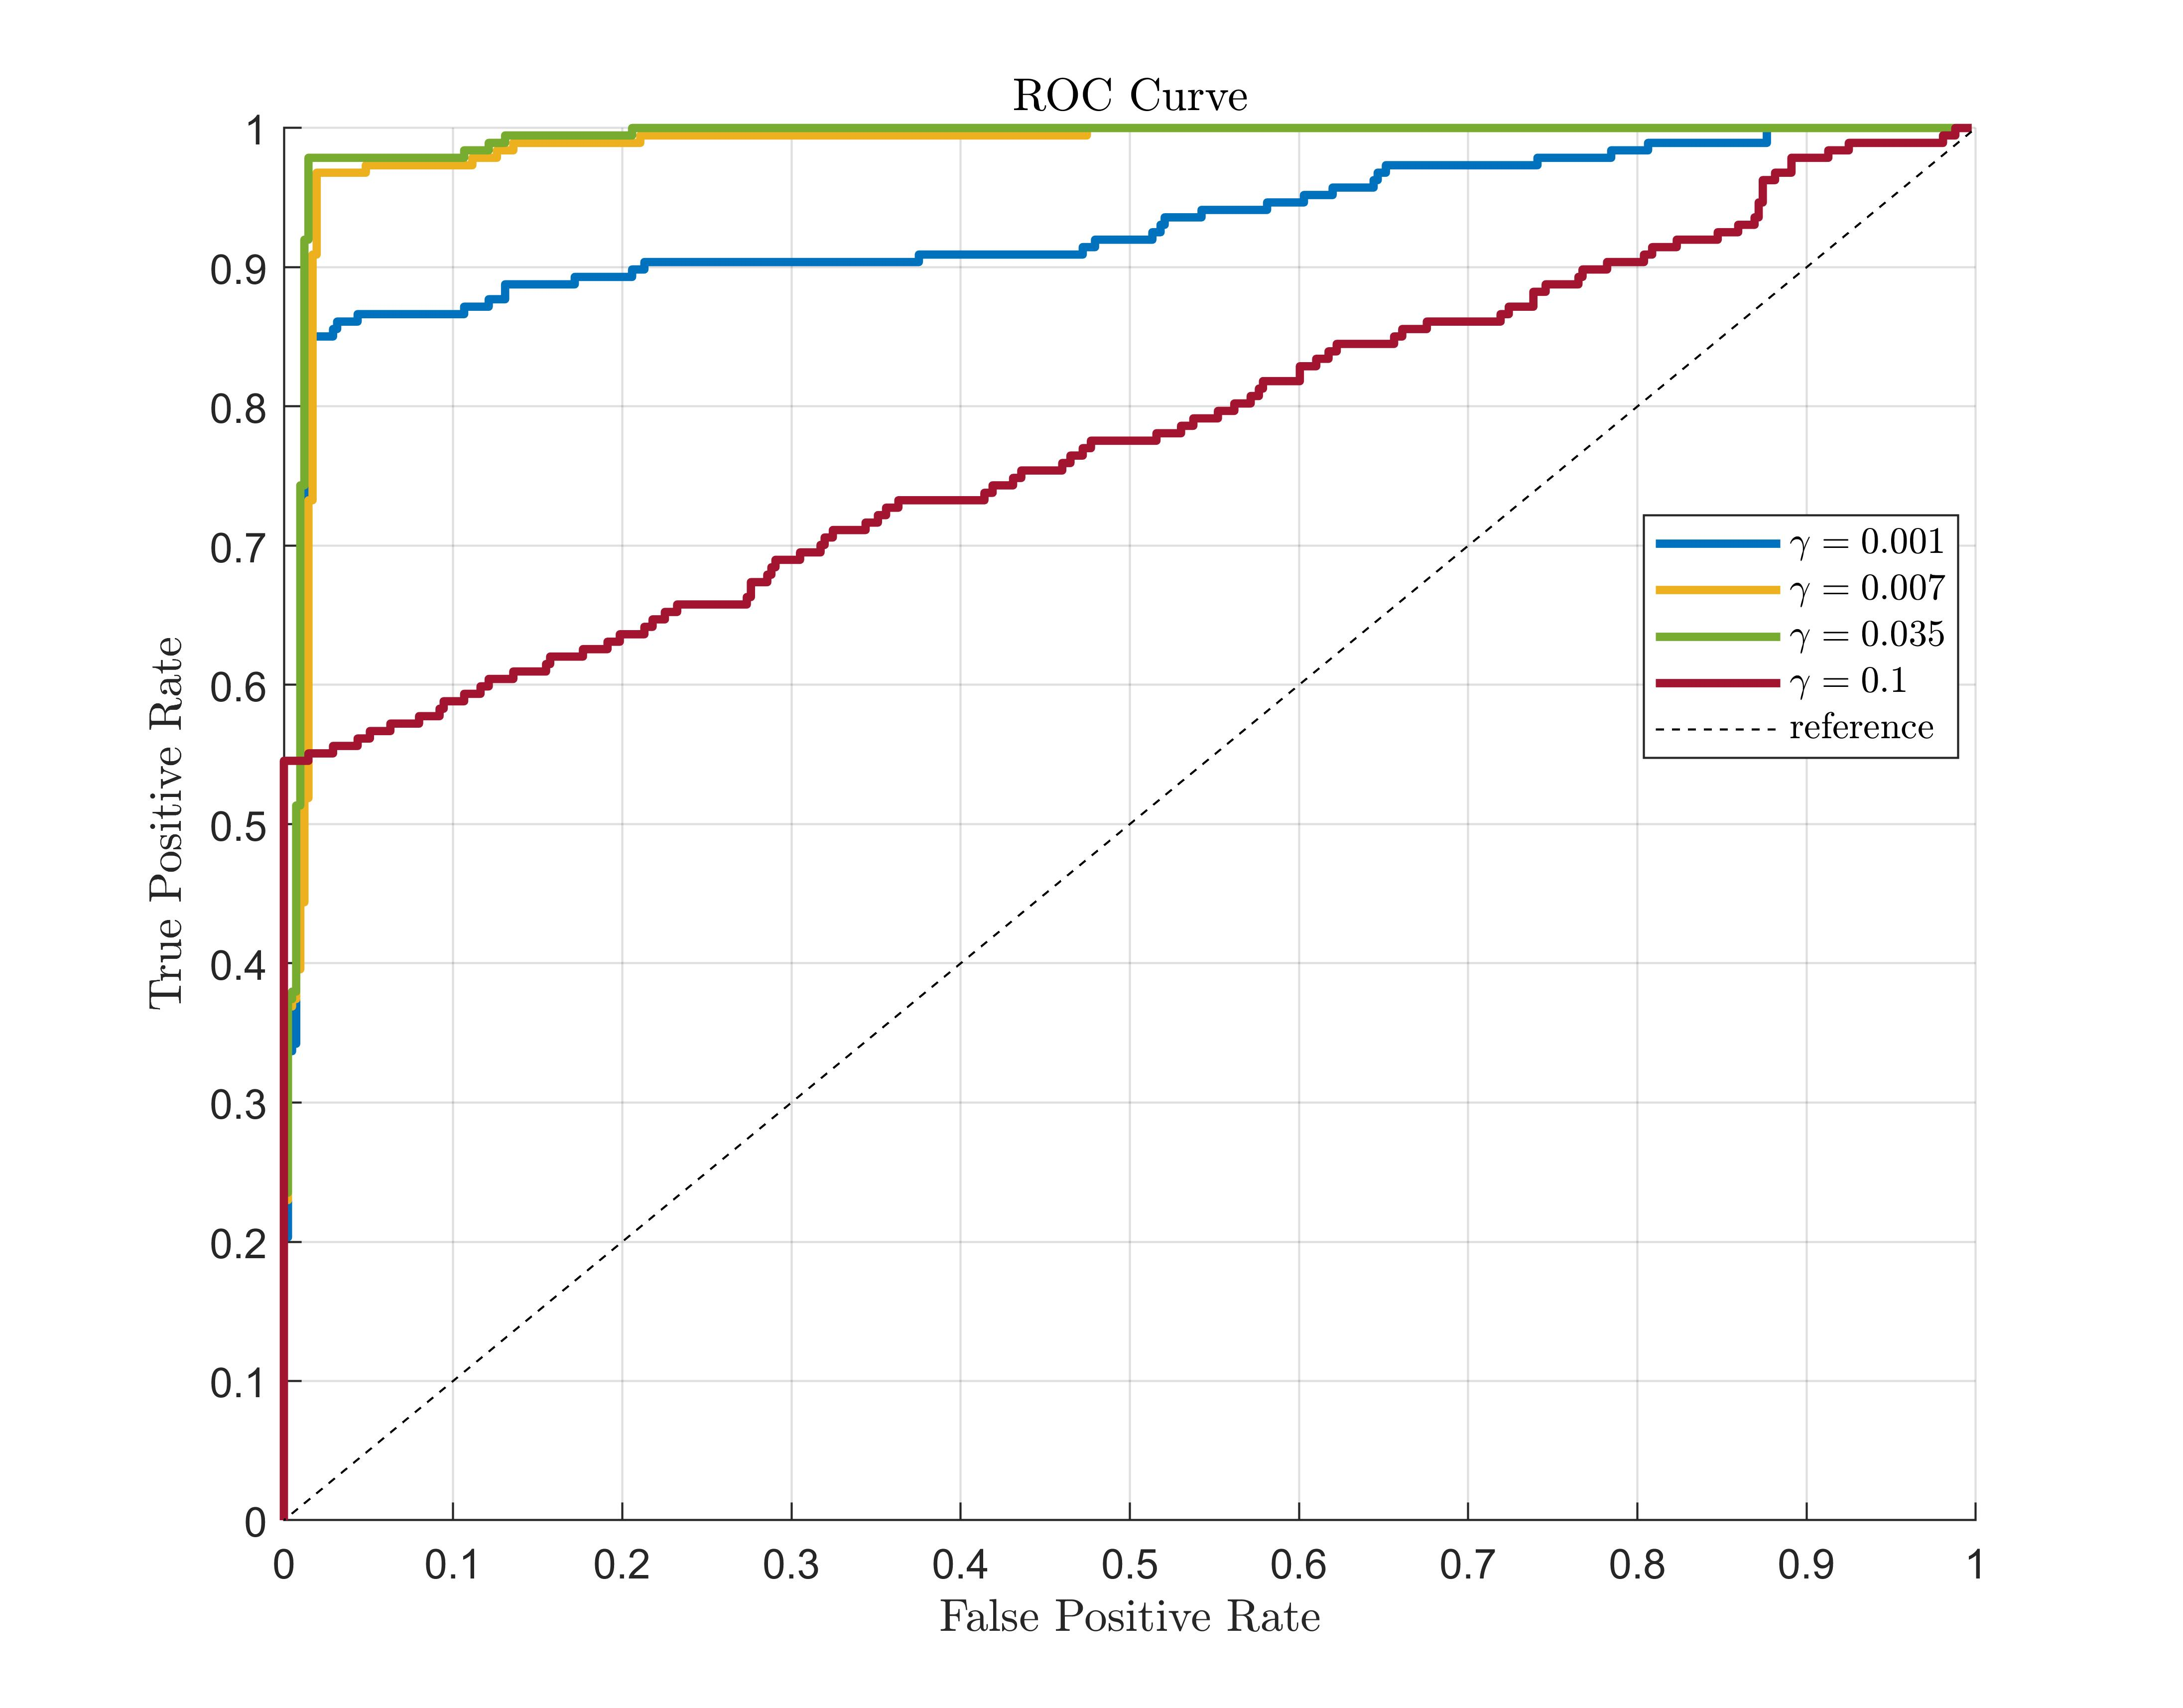
\includegraphics[width=0.88\textwidth]{FT.jpg}
	\caption{ROC Curves vs Different Choices of Gamma $\gamma$ in SVM(RBF)}
	\label{fig:ft}
\end{figure}

\begin{figure}[!htbp]
	\centering
	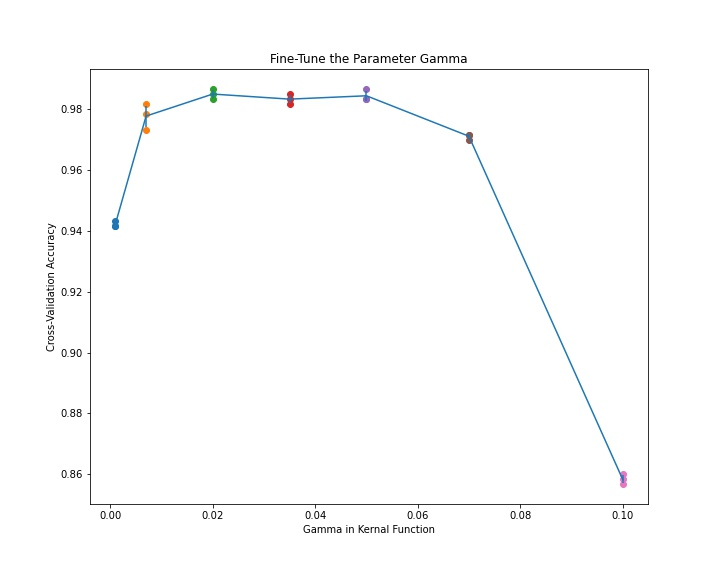
\includegraphics[width=0.88\textwidth]{FT2.jpg}
	\caption{Cross-Validation Accuracy vs Different Choices of Gamma $\gamma$ in SVM(RBF)}
	\label{fig:ft2}
\end{figure}

\hspace{0.7cm}
As we can observe, the cross-validation accuracy and AUC will climb up initially as we increase the value of $\gamma$, followed a stable peak period, and finally, the cross-validation accuracy and AUC will drop dramatically. Therefore, the hyperparameter $\gamma$ should be chosen between $0.02$ and $0.05$, which can make the SVM with RBF kernal performs the best on this partial MNIST dataset.



\end{document}
